\textbf{2.1.1.} 一导体球壳内是球形空腔, 空腔的中心有一电荷量为 $q_{2}$ 的点电荷, 球

壳外离球心为 r 处有一电荷量为 $q_{1}$ 的点电荷, 如图 2.1.1 所示. 已知导体球壳上所有电荷量的代数和为零. 试求: (1) $q_{1}$ 作用在 $q_{2}$ 上的力; (2) $q_{2}$ 所受的力.

\vfill

\textbf{2.1.2.} 一金属球内有两个球形空腔，两空腔中心相距为 $a$ ，它们的联线通过球心；在两腔中心各有一个点电荷，电荷量分别为 $q_{1}$ 和 $q_{2}$ 。球外有一电荷量为 $q$ 的点电荷，处在 $q_{2}$ 到 $q_{1}$ 的延长线上，到 $q_{1}$ 的距离为 $b$ ，如图2.1.2所示。已知金属球上所有电荷量的代数和为零. 试求金属球上的电荷作用在 $q_{2}$ 上的力.

图2.1.2
\begin{center}
    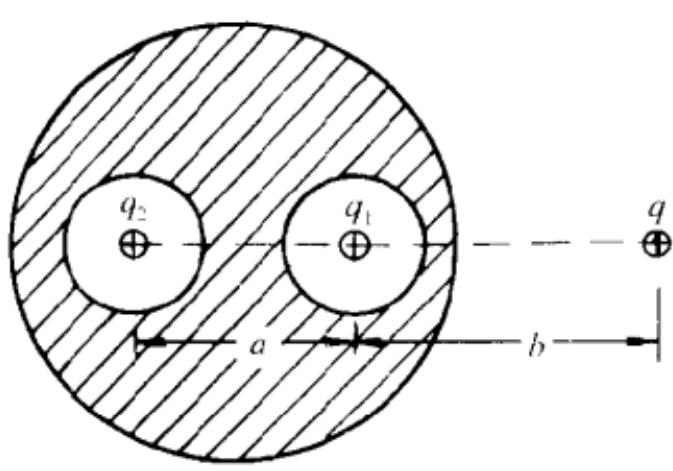
\includegraphics[width=0.5\linewidth]{figures/fig_2_1_2.jpg}
\end{center}

\vfill

\newpage

\textbf{2.1.3.} 两金属球壳 $A$ 和 $B$ 中心相距为 $r, A$ 和 $B$ 原来都不带电。现在 $A, B$ 的中心各放一个点电荷，电荷量分别为 $q_{1}$ 和 $q_{2}$ ，如图2.1.3所示。（1）试求 $q_{1}$ 作用在 $q_{2}$ 上的力。 $q_{2}$ 有加速度吗？(2)去掉金属壳 $B$ ，试求 $q_{1}$ 作用在 $q_{2}$ 上的力。这时 $q_{2}$ 有加速度吗？

\vfill

\textbf{2.1.4.} 我们通常说,在静电平衡时,导体内部的电场强度处处为零.但是,由于导体是由原子核和电子构成的,而原子核是不连续的,因此,在靠近原子核的地方,必然存在很强的电场.你怎样看待这个矛盾?

【解答】在电磁学里,我们所涉及的量如电荷量密度 $\rho$ 、电场强度 $E$ 、电势 $U$ 等,除特别指明者外,一般都是宏观量,它们都是对宏观小而微观大的区域统计平均的结果。通常说导体内部电场强度处处为零,指的是宏观电场;而“靠近原子核的地方有很强的电场”,则指的是微观电场。一个不带电的导体,在静电平衡时,从微观上看,其中有原子核,核外有电子,显然,各点的电荷量密度和电场强度彼此相差很大;但对于一个宏观小而微观大的区域(例如线度小于 $10^{-5}$ 米和大于 $10^{-8}$ 米的区域)来说,平均起来,则处处电荷量密度 $\rho = 0$ ,电场强度 $E = 0$ 。关于这些,可参看 J.D. 杰克逊著(朱培豫译),《经典电动力学》上册(人民教育出版社,1979),250页。

\vfill

\newpage

\textbf{2.1.5.} 有人说：“在静电情况下，导体带电有两条规律：(1)电荷只分布在外表面上，内表面上无电荷；(2)电荷量的面密度与该处表面的曲率半径成反比。”你认为他说的这两点对不对？为什么？

【解答】（1）不一定对。在导体里面的空腔里如果有电荷，则空腔的表面（即导体的内表面）上便有电荷，只有在空腔内无电荷时，空腔的表面上才无电荷。

(2)不对. 导体表面某处的曲率半径越小, 则该处电荷量的面密度就越大, 但不一定是反比关系. 还有, 导体表面某处电荷量的面密度不仅与该处的曲率半径有关, 还与周围环境有关, 关系是很复杂的.

\vfill

\textbf{2.1.6.} 一个有厚度的金属球壳带有电荷量 q，现在它的中心放一个电荷量为 -q 的点电荷，试问：(1) 金属球壳上电荷如何分布？(2) 这与“导体上的电荷只分布在外表面上”的结论有无矛盾？(3) 导体带电时，在什么情况下电荷才完全分布在外表面上？

【解答】（1）由对称性、高斯定理和电荷量守恒得出：球壳的外表面上无电荷，内表面上均匀地分着电荷量为 $-q$ 的电荷.

(2)无矛盾.“导体上的电荷只分布在外表面上”的结论是有条件的,这条件是:导体空腔内无电荷.

(3)导体的空腔内没有电荷.

\vfill

\newpage

\textbf{2.1.7.} 一导体球壳 $A$ 带有电荷量 $q_{A} = -1 \times 10^{-6}$ 库仑, 导体小球 $B$ 带有电荷量 $q_{B} = 2 \times 10^{-6}$ 库仑. 用丝线吊着小球 $B$ , 经 $A$ 上的小孔放入 $A$ 内. (1) $B$ 不与 $A$ 接触, 令 $A$ 瞬时接地, 如图 2.1.7(1) 所示, 然后断开接地, 再把 $B$ 取出. 问 $A$ 、 $B$ 的带电情况各如何? (2) 如图 2.1.7(2) 所示, $B$ 与 $A$ 的内壁接触, $A$ 不接地, 然后把 $B$ 取出. 问这时 $A$ 、 $B$ 的带电情况各如何?

【解答】(1) A 带的电荷量为 $q_{A}^{\prime} = -q_{B} = -2 \times 10^{-6}$ 库仑. 分布在外表面上; B 带的电荷量

$q_{B}^{\prime} = q_{B} = 2\times 10^{-6}$ 库仑.

(2) A 带的电荷量为 $q_{A}^{\prime\prime}=q_{A}+q_{B}=1\times10^{-6}$ 库仑，分布在外表面上；B 带的电荷量为 $q_{B}^{\prime\prime}=0$ .

(1)

图2.1.7
(2)

图2.1.8
\begin{center}
    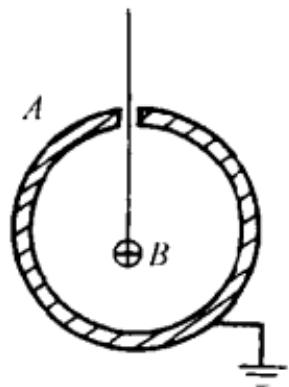
\includegraphics[width=0.5\linewidth]{figures/fig_2_1_7_1.jpg}
\end{center}
\begin{center}
    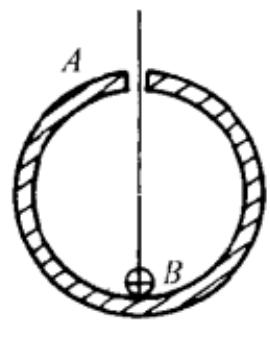
\includegraphics[width=0.5\linewidth]{figures/fig_2_1_7_2.jpg}
\end{center}
\begin{center}
    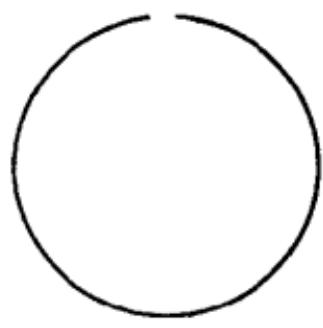
\includegraphics[width=0.5\linewidth]{figures/fig_2_1_7_3.jpg}
\end{center}

\vfill

\textbf{2.1.8.} 金属薄球壳上有一小孔(图 2.1.8)，当它带电时，在静电平衡的情况下，内表面上有电荷吗？

【解答】内表面上有电荷,但很少;孔越小,内表面上的电荷越少. 汤姆孙(W. Thomson, 即开尔文)曾计算过电荷分布的情况,参见 J.H.Jeans, The Mathematical Theory of Electricity and Magnetism, 5th ed., 1951, pp.250\~251.

\vfill

\newpage

\textbf{2.1.9.} 在静电情况下,为什么一条电力线的两端不能在同一导体上?

【解答】在静电情况下,导体是等势体,它上面任何两点的电势都相等.电力线是沿电场强度 E 的方向画出的曲线,它从高电势走向低电势,所以它上面任何两点的电势都不相等.因此,在静电情况下,一条电力线的两端不可能在同一导体上.

\vfill

\textbf{2.1.10.} 真空中有一组彼此不接触的带电导体,试论证:电势的极大值或极小值只能出现在这些导体上.

【论证】由高斯定理得出：

$$
\nabla \cdot \boldsymbol {E} = \frac {\rho}{\varepsilon_ {0}}\tag{1}
$$

式中 $\rho$ 是电荷密度.

因为

$$
\boldsymbol {E} = - \nabla U\tag{2}
$$

所以

$$
\nabla^ {2} U = - \frac {\rho}{\varepsilon_ {0}}\tag{3}
$$

用笛卡儿坐标系表示,即

$$
\frac {\partial^ {2} U}{\partial x ^ {2}} + \frac {\partial^ {2} U}{\partial y ^ {2}} + \frac {\partial^ {2} U}{\partial z ^ {2}} = - \frac {\rho}{\varepsilon_ {0}}\tag{4}
$$

电势的极大值 $U_{max}$ 出现的地方必须是

$$
\frac {\partial^ {2} U}{\partial x ^ {2}} <   0, \quad \frac {\partial^ {2} U}{\partial y ^ {2}} <   0, \quad \frac {\partial^ {2} U}{\partial z ^ {2}} <   0\tag{5}
$$

电势的极小值 $U_{\min}$ 出现的地方必须是

$$
\frac {\partial^ {2} U}{\partial x ^ {2}} > 0, \quad \frac {\partial^ {2} U}{\partial y ^ {2}} > 0, \quad \frac {\partial^ {2} U}{\partial z ^ {2}} > 0\tag{6}
$$

现在在导体外没有电荷，故由式(4)得出：在导体以外的空间里有

$$
\frac {\partial^ {2} U}{\partial x ^ {2}} + \frac {\partial^ {2} U}{\partial y ^ {2}} + \frac {\partial^ {2} U}{\partial z ^ {2}} = 0\tag{7}
$$

式(7)既不满足式(5)，也不满足式(6). 这就表明：在导体以外的空间里，电势既不可能有极大值，也不可能有极小值. 换句话说，电势的极大值或极小值只能出现在导体上.

\vfill

\newpage

\textbf{2.1.11.} 有一些互相绝缘的不带电导体 A、B、C、…，它们的电势都是零。现在使其中任一个导体 A 带正电荷，试论证：(1) 所有这些导体的电势都高于零；(2) 其他导体的电势都低于 A 的电势。

图2.1.11

【论证】如图2.1.11，A带正电荷，B、C、…必都因静电感应而出现感应电荷。这时，必有电力线从A出发，有的到达B、C、…等上，有的去向无穷远。故A的电势高于零（以无穷远处电势为零），A的电势高于B、C、…等。而B、C、…等上因感应而出现的正电荷，也会有电力线从它们出发，这些电力线只能到达电势较低的导体上或去向无穷远。从电势最低的导体上发出的电力线，便只能去向无穷远了；所以电势最低的导体其电势也高于零，因而所有导体的电势都高于零。
\begin{center}
    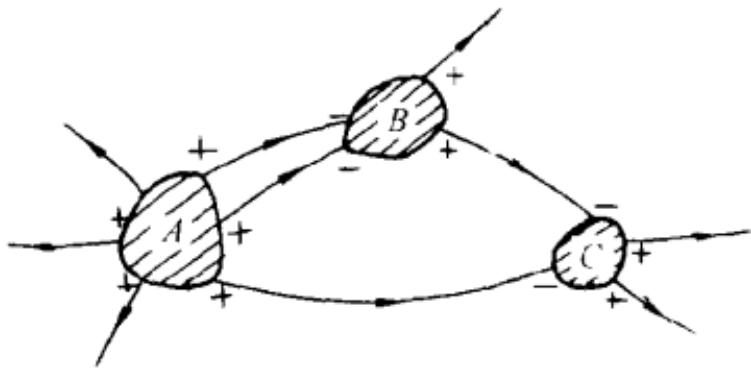
\includegraphics[width=0.5\linewidth]{figures/fig_2_1_11.jpg}
\end{center}

\vfill

\textbf{2.1.12.} 两导体上分别带有电荷量 $2q$ 和 $-q, q > 0$ , 它们都处在一个封闭的金属壳内. 试论证: 电荷量为 $2q$ 的导体其电势高于金属壳的电势.

【论证】设电荷量 q 发出 N 条电力线，则 2q 的导体便要发出 2N 条电力线，而 -q 的导体则应有净 N 条电力线终止在它上面。因此，2q 的导体上必有电力线直到金属壳的内表面上，如图 2.1.12 所示。故知 2q 的导体的电势高于金属壳的电势。

图2.1.12

图2.1.13
\begin{center}
    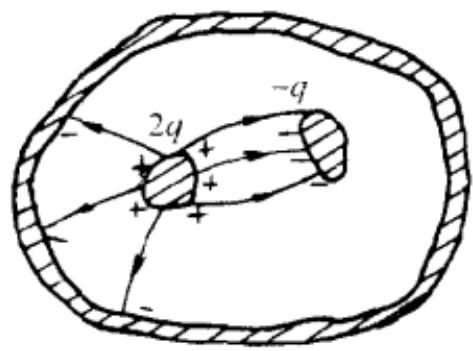
\includegraphics[width=0.5\linewidth]{figures/fig_2_1_12_1.jpg}
\end{center}
\begin{center}
    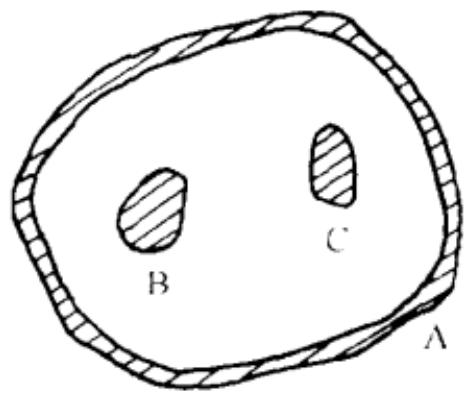
\includegraphics[width=0.5\linewidth]{figures/fig_2_1_12_2.jpg}
\end{center}

\vfill

\newpage

\textbf{2.1.13.} 如图 2.1.13, 一封闭的导体壳 A 内有两个导体 B 和 C, 它们都不带电. 现在设法让 B 带上正电. 试论证: B 的电势 $U_{B}$ 高于 C 的电势 $U_{C}, C$ 的电势又高于 A 的电势 $U_{A}$ , 而 $U_{A} > 0$ , 即 $U_{B} > U_{C} > U_{A} > 0$ .

【论证】 $B$ 带正电， $A$ 和 $C$ 上必因感应而出现负电荷和正电荷，必定有电力线从 $B$ 到达 $C$ 和从 $B$ 到达 $A$ 。故知 $U_B > U_C, U_B > U_A$ 。又 $C$ 上的正电荷要发出电力线，这些电力线既不能到达 $B$ 上，又不能在空间中断，只能到达导体壳 $A$ 上。故知 $U_C > U_A$ 。又因为 $A$ 原来不带电，现在它的空腔里 $B$ 带正电，故 $A$ 的外表面上必有正电荷，因而有电力线从 $A$ 出发，直向无穷远去，故知 $U_A > 0$ （以无穷远处电势为零）。于是得 $U_B > U_C > U_A > 0$ 。

\vfill

\textbf{2.1.14.} 真空中有一个不带电的导体球, 现在把电荷量为 q 的点电荷放在球外离球心为 a 处, 试求这时导体球的电势.

\vfill

\newpage

\textbf{2.1.15.} 半径为 r 的导体球带有电荷量 Q，现将一些点电荷放在球外，它们的电荷量分别为 $q_{1}, q_{2}, \cdots, q_{n}$ ，到球心的距离分别为 $r_{1}, r_{2}, \cdots, r_{n}$ 。试求这时导体球的电势。

\vfill

\textbf{2.1.16.} 电荷量为 q 的点电荷, 放在半径为 R 的导体球外离球心为 a 处, 测得这时导体球的电势为零(即等于无穷远处的电势). 试求导体球上的电荷量.

\vfill

\newpage

\textbf{2.1.17.} 带有电荷量 Q 的导体球壳, 内外半径分别为 $R_{1}$ 和 $R_{2}$ , 现将电荷量为 $q_{1}$ 的点电荷放在壳内离球心 O 为 $r_{1}$ 处, 电荷量为 $q_{2}$ 的点电荷放在壳外离球心 O 为 $r_{2}$ 处, 如图 2.1.17 所示. 试求球心 O 的电势.

\vfill

\textbf{2.1.18.} 一半径为 a 的导体球带有电荷量 Q，现将一半径为 b 的均匀带电圆环放在球旁边，圆环的轴线通过球心，环心到球心的距离为 r，环上的电荷量为 q，如图 2.1.18 所示。试求导体球的电势。

\vfill

\newpage

\textbf{2.1.19.} 平行板电容器充电后,两极板 A 和 B 上电荷量的面密度分别为 $\sigma$ 和 $-\sigma$ , 如图 2.1.19 所示. 设 P 为两板间任一点, 略去两极板的边缘效应. (1) 试求 A 板上的电荷在 P 点产生的电场强度 $E_{A}$ ; (2) 试求 B 板上的电荷在 P 点产生的电场强度 $E_{B}$ ; (3) 试求 A、B 两板上的电荷在 P 点产生的电场强度 E; (4) 若把 B 板拿走, 试求 A 板上的电荷在 P 点产生的电场强度.
\begin{center}
    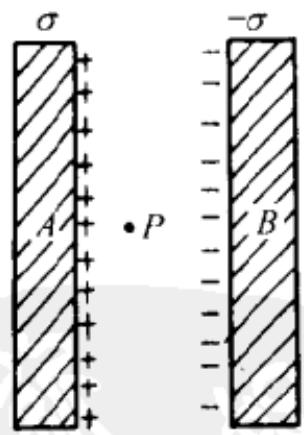
\includegraphics[width=0.5\linewidth]{figures/fig_2_1_19.jpg}
\end{center}

\vfill

\textbf{2.1.20.} 试证明:对于两个无限大的平行平面带电导体板(图2.1.20)来说,(1)相向的两面(图中2和3)上,电荷量的面密度总是大小相等而符号相反;(2)相背的两面(图中1和4)上,电荷量的面密度总是大小相等而符号相同.

\vfill

\newpage

\textbf{2.1.21.} 两块大小相同的平行金属板,带有相同的电荷量,略去边缘效应.试证明:(1)若它们的电荷同号,则电荷便只分布在相背的两面上;(2)若它们的电荷异号,则电荷便只分布在相向的两面上.

\vfill

\textbf{2.1.22.} 两块大小相同的平行金属板,所带的电荷量不相等,如 $Q_{1} > Q_{2}$ (图2.1.22). 略去边缘效应,试证明:(1)相向的两面上,电荷量的面密度大小相等而符号相反;相背的两面上,电荷量的面密度大小相等而符号相同;(2)相向面上的电荷量分别为 $\frac{1}{2}(Q_1 - Q_2)$ 和 $\frac{1}{2}(Q_2 - Q_1)$ , 相背面上的电荷量均为 $\frac{1}{2}(Q_1 + Q_2)$ .
\begin{center}
    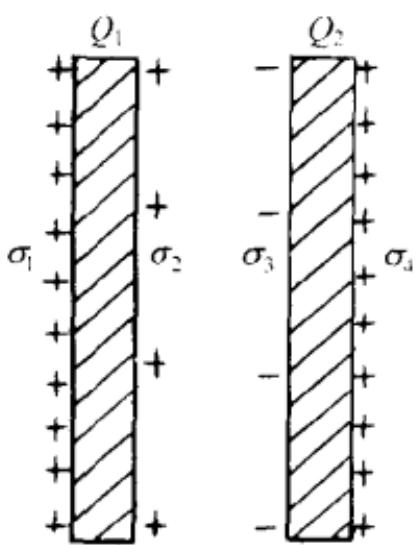
\includegraphics[width=0.5\linewidth]{figures/fig_2_1_22.jpg}
\end{center}

\vfill

\newpage

\textbf{2.1.23.} 两带电的金属平行板所带电荷量大小相等,但符号相反.已知两板的面积都是 $3.6cm^{2}$ ,相距为1.6mm,电势差为120V.略去边缘效应,试求两板间的电场强度和各板上所带的电荷量.

\vfill

\textbf{2.1.24.} 两平行金属板 A、B 带有等量异号电荷，相距为 5.0mm，两板的面积都是 $150cm^{2}$ ，电荷量的大小都是 $2.66 \times 10^{-8}C$ ，A 板带正电并接地，如图 2.1.24 所示。以地的电势为零，并略去边缘效应，试问：B 板的电势是多少？A、B 间离 A 板 1.0mm 处的电势是多少？

【解答】根据前面2.1.21题的结果， $A, B$ 两板上的电荷都均匀分布在相向的两面上。由高斯定理得出，两板间的电场强度为


$$
E = \frac {\sigma}{\varepsilon_ {0}} e = \frac {Q}{\varepsilon_ {0} S} e\tag{1}
$$

图2.1.24

式中 Q 是每个板上电荷量的大小, S 是板的面积, e 是垂直于板面的单位矢量, 方向从 A 到 B. 由式(1)得 B 板的电势为

$$
\begin{array}{r l} U _ {B} & = U _ {A} - \int_ {A} ^ {B} \boldsymbol {E} \cdot \mathrm{d} \boldsymbol {l} = 0 - \int_ {A} ^ {B} E \mathrm{d} l = - \frac {Q l}{\varepsilon_ {0} S} \\ & = - \frac {2 . 6 6 \times 1 0 ^ {- 8} \times 5 . 0 \times 1 0 ^ {- 3}}{8 . 8 5 4 \times 1 0 ^ {- 1 2} \times 1 5 0 \times 1 0 ^ {- 4}} \\ & = - 1. 0 \times 1 0 ^ {3} (\mathrm{V}) \end{array}\tag{2}
$$

$A, B$ 间离 $A$ 板 $1.0\mathrm{mm}$ 处的电势为

$$
\begin{array}{r l} {U = - \int_ {A} ^ {P} E d l = - E l _ {P} = - U _ {B} \frac {l _ {P}}{l} = - 1. 0 \times 1 0 ^ {3} \times \frac {1 . 0}{5 . 0}} \\ & {= - 2. 0 \times 1 0 ^ {2} (\text {伏})} \end{array}
$$
\begin{center}
    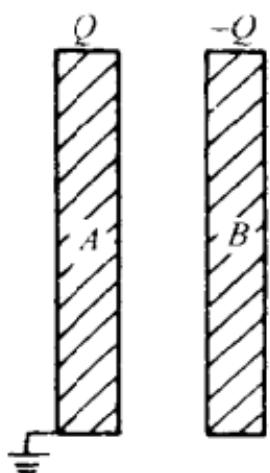
\includegraphics[width=0.5\linewidth]{figures/fig_2_1_24.jpg}
\end{center}

\vfill

\newpage

\textbf{2.1.25.} 三块平行的金属板 A、B 和 C，面积都是 $200 \, cm^{2}$ ，A、B 相距 4.0 mm，

图2.1.25

A、C相距2.0mm，B和C都接地，如图2.1.25所示。如果使A板带 $3.0\times10^{-7}C$ 的正电荷量，在略去边缘效应时，试问B、C两板上的感应电荷量各是多少？以地的电势为零，A板的电势是多少？
\begin{center}
    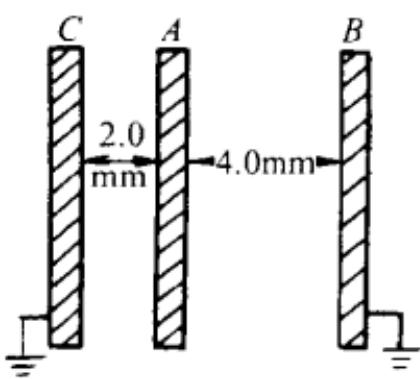
\includegraphics[width=0.5\linewidth]{figures/fig_2_1_25.jpg}
\end{center}

\vfill

\textbf{2.1.26.} 一平行板电容器两极板的面积都是 S，相距为 d，分别维持电势 $U_{A}=U$ 和 $U_{B}=0$ 不变。现将一块带有电荷量 q 的导体薄片（其厚度可略去不计）放在两极板的正中间，薄片的面积也是 S，如图 2.1.26 所示。略去边缘效应，试求薄片的电势。
\begin{center}
    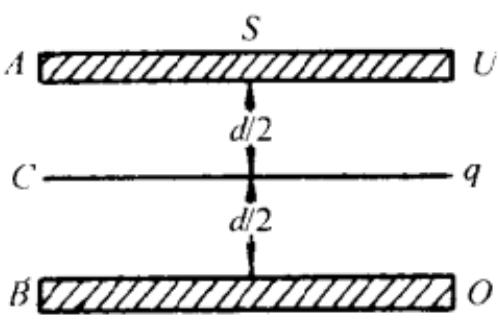
\includegraphics[width=0.5\linewidth]{figures/fig_2_1_26.jpg}
\end{center}

\vfill

\newpage

\textbf{2.1.27.} 半径为 $a$ 的导体球带有电荷量 $q, q$ 均匀分布在球面上。试求离球心为 $r$ 处的电场强度和电势。

\vfill

\textbf{2.1.28.} 直径为 1.0m 的金属球带有正电荷量 $1.0\mu C$ . 试求球面上和离球面

1.0m 处的电势.

\vfill

\newpage

\textbf{2.1.29.} 一导体球半径为 R，电势为 U。（1）试求它上面电荷量的面密度 $\sigma$ ；(2) 计算 R = 0.15m, U = 200V 时 $\sigma$ 的值.

\vfill

\textbf{2.1.30.} 内外半径分别为 $R_{2}$ 和 $R_{3}$ 的金属球壳 $B$ 带有电荷量 $Q$ ，在它里面放一个带有电荷量 $q$ 、半径为 $R_{1}$ 的同心金属球 $A$ ，如图2.1.30所示。（1）试求离球心为 $r$ 处的电场强度 $\pmb{E}$ 和电势 $U$ 以及球与壳的电势差；(2)试画出 $E - r$ 曲线和 $U - r$ 曲线；(3)当 $q = -Q$ 时各处的 $\pmb{E}$ 和 $U$ 如何？
\begin{center}
    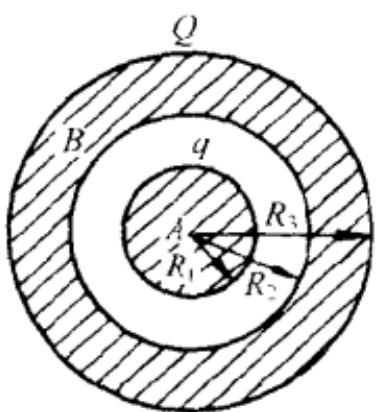
\includegraphics[width=0.5\linewidth]{figures/fig_2_1_30.jpg}
\end{center}

\vfill

\newpage

\textbf{2.1.31.} 三个不带电的同心导体薄球壳, 它们的厚度都可略去不计, 它们的半径分别为 $2r, 4r$ 和 $6r$ ; 现在球心放一个电荷量为 $Q$ 的点电荷, 如图 2.1.31 所示. 图中 $A, B, C$ 三点到球心的距离分别为 $r, 3r$ 和 $5r$ . 试问在三个导体球壳上分别放上多少电荷量, 能够使 $A, B, C$ 三点的电场强度的大小都相等?
\begin{center}
    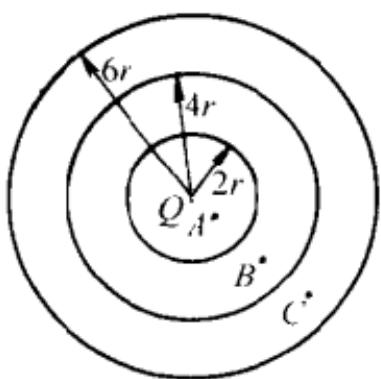
\includegraphics[width=0.5\linewidth]{figures/fig_2_1_31.jpg}
\end{center}

\vfill

\textbf{2.1.32.} 半径为 $R_{1}$ 的金属球带有电荷量 q，它外面有一个和它同心的金属球壳，壳的内外半径分别为 $R_{2}$ 和 $R_{3}$ ，如图2.1.32所示。已知球壳的电势为零。（1）试求离球心为 r 处的电场强度 E 和电势 U 以及球与壳的电势差；（2）画出 E-r 和 U-r 曲线。

\vfill

\newpage

\textbf{2.1.33.} 半径为 $R_{1}$ 的导体球外有同心的导体球壳, 壳的内外半径分别为 $R_{2}$ 和 $R_{3}$ , 如图 2.1.33 所示; 已知球壳带有电荷量 Q, 球的电势为零. 试求球上的电荷量和球壳的电势.

\vfill

\textbf{2.1.34.} 同轴传输线由很长的圆柱形长直导线和套在它外面的同轴导体圆管构成,导线的半径为 $R_{1}$ , 电势为 $U_{1}$ , 圆管的内半径为 $R_{2}$ , 电势为 $U_{2}$ , 如图 2.1.34 所示. 试求它们之间离轴线为 r 处 ( $R_{1} < r < R_{2}$ ) 的电势.

\vfill

\newpage

\textbf{2.1.35.} 一很长的直导线横截面的半径为 $a$ ，它外面套有内半径为 $b$ 的同轴导体圆筒，两者互相绝缘。已知导线的电势为 $U$ ，圆筒接地，以地的电势为零，试求导线与圆筒间的电场强度以及圆筒的上电荷量的面密度。

\vfill

\textbf{2.1.36.} 电子二极管由两个同轴的金属直圆筒构成,内筒是发射电子的阴极 $K$ ,它的外半径为 $1.0 \mathrm{~mm}$ ;外筒是接收电子的阳极 $A$ ,它的内半径为 $1.0 \mathrm{~cm}$ ,板压(即阳极与阴极的电势差)为 $300 \mathrm{~V}$ ,如图2.1.36所示.略去边缘效应.试求:(1)阴极外表面上电荷量的面密度;(2)电子刚离开阴极时所受的力;(3)电子到达阳极时的速度.已知电子的质量为 $9.11 \times 10^{-31} \mathrm{~kg}$ ,电荷的大小为 $1.60 \times 10^{-19} \mathrm{C}$ ,电子离开阴极时速度可当作是零.
\begin{center}
    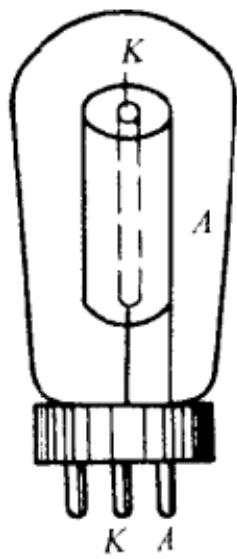
\includegraphics[width=0.5\linewidth]{figures/fig_2_1_36.jpg}
\end{center}

\vfill

\newpage

\textbf{2.1.37.} 试证明: 若导体表面上某处电荷量的面密度为 $\sigma$ , 则在该导体外很靠

近 $\sigma$ 处，电场强度为 $E = \frac{\sigma}{\varepsilon_0}\pmb{n}$ ，式中 $\pmb{n}$ 是 $\sigma$ 处导体外法线方向上的单位矢量。

\vfill

\textbf{2.1.38.} 试证明:导体表面上某处电荷量的面密度为 $\sigma$ 时,该处导体单位面积所受的力为 $\frac{\sigma^{2}}{2\varepsilon_{0}}n,n$ 是该处导体表面外法线方向上的单位矢量.

\vfill

\newpage

\textbf{2.1.39.} 实验表明,在靠地面处有相当强的静电场,E垂直于地面向下,其大小约为100V/m.试求:(1)地面上电荷量的面密度;(2)地面每平方米所受的静电力.

\vfill

\textbf{2.1.40.} 一带电的肥皂泡半径为 R，电势为 U，肥皂水的表面张力系数为 $\alpha$ 。当吹肥皂泡的小管与大气相通时，泡内外的空气压强相同，设这时肥皂泡处于稳定状态，略去小管的影响，把肥皂泡当作一个带电的球壳，试求 R、U 和 $\alpha$ 之间的关系。

\vfill

\newpage

\textbf{2.1.41.} 一肥皂泡的半径为 $r$ ，肥皂水的表面张力系数为 $\alpha$ ，外部空气的压强为 $p$ 。使这肥皂泡带上电荷量 $q$ 后，它的半径增大为 $R$ 。试证明： $(R^3 - r^3)p + 4\alpha (R^2 - r^2) = \frac{q^2}{32\pi^2\varepsilon_0R}$ 。

\vfill

\textbf{2.1.42.} 一不带电的肥皂泡半径为 $R$ ，肥皂水的表面张力系数为 $\alpha$ ，外面大气压强为 $p$ 。试证明：要使这肥皂泡的半径增大一倍，它需要带的电荷量为 $Q = 8\pi \sqrt{\varepsilon_0 R^3 (7pR + 12\alpha)}$ 。

\vfill

\newpage

\textbf{2.1.43.} 在一金属球外,有一同心的金属球壳,壳的内外半径分别为 a 和 b,这壳由互相密切接触的两部分 A 和 B 组成, 它们的交界面是一个平面, 这平面到球心的距离为 c, 如图 2.1.43 所示. 球和壳原来都不带电, 现在让球带电. 试证明: 当 $c < \frac{ab}{\sqrt{a^{2} + b^{2}}}$ 时, B 所受的静电力是吸引力.
\begin{center}
    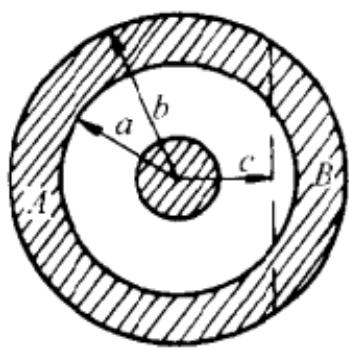
\includegraphics[width=0.5\linewidth]{figures/fig_2_1_43.jpg}
\end{center}

\vfill

\textbf{2.1.44.} 电荷量为 q 的点电荷, 到一无穷大导体平面的距离为 l, 如图 2.1.44 所示. 已知导体的电势为零, 试求导体表面上的电荷量分布.

图2.1.44

图2.1.44(1)
\begin{center}
    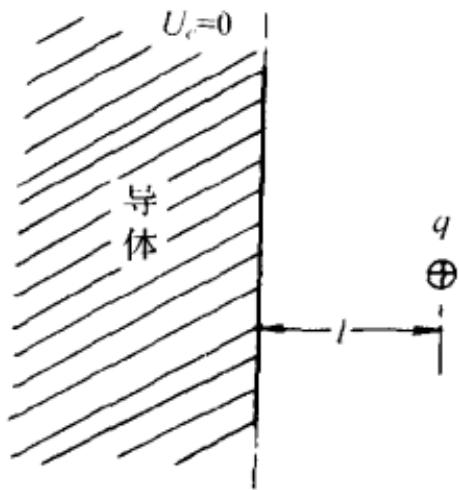
\includegraphics[width=0.5\linewidth]{figures/fig_2_1_44_1.jpg}
\end{center}
\begin{center}
    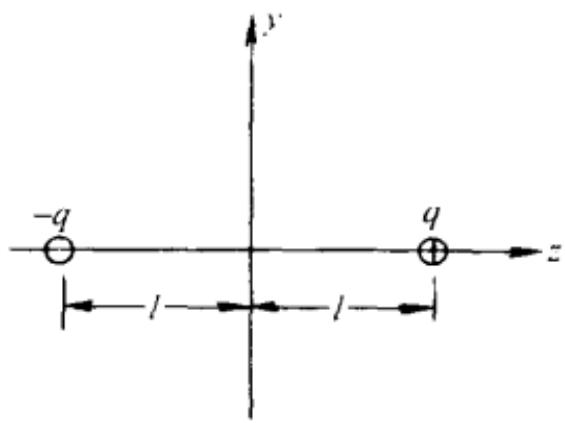
\includegraphics[width=0.5\linewidth]{figures/fig_2_1_44_2.jpg}
\end{center}

\vfill

\newpage

\textbf{2.1.45.} 电荷量为 q 的点电荷到一无穷大导体平面的距离为 l，已知导体的电势为零。电力线从 q 发出时，有些是与导体平面平行的，试问这些电力线在何处碰到导体表面？

\vfill

\textbf{2.1.46.} 半径为 $R$ 的金属球带有电荷量 $Q$ , 将电荷量为 $q$ 的一个点电荷放在离球心为 $a$ 处, 如图 2.1.46(1) 所示. 试求球上电荷作用在 $q$ 上的力.

图2.1.46(1)

图2.1.46(2)
\begin{center}
    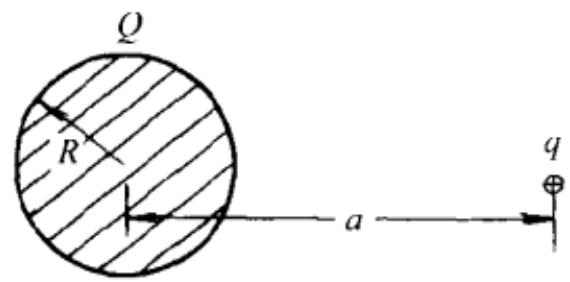
\includegraphics[width=0.5\linewidth]{figures/fig_2_1_46_1.jpg}
\end{center}
\begin{center}
    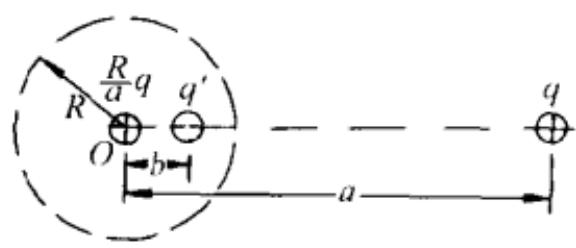
\includegraphics[width=0.5\linewidth]{figures/fig_2_1_46_2.jpg}
\end{center}

\vfill

\newpage

\textbf{2.2.1.} 将电荷量分别为 $q_{1}$ 和 $q_{2}$ 的两个自由点电荷，放在电容率为 $\varepsilon$ 的无穷大均匀介质中，当它们都静止时，相距为 $r$ 。试求：(1) $q_{1}$ 作用在 $q_{2}$ 上的力；(2) $q_{2}$ 所受的力。

\vfill

\textbf{2.2.2.} 将电荷量为 q 的自由点电荷放在电容率为 $\varepsilon$ 的无穷大均匀介质中，试求 r 处 P 点(图 2.2.2)的电场强度.

\vfill

\newpage

\textbf{2.2.3.} 一平行板电容器两极板间充满了电容率为 $\varepsilon$ 的均匀介质, 已知两极板上电荷量的面密度分别为 $\sigma$ 和 $-\sigma$ , 如图2.2.3所示. 略去边缘效应. 试求介质中的电场强度 $E$ 、极化强度 $P$ 、电位移 $D$ 、极化电荷量密度 $\rho'$ 和极化电荷量的面密度 $\sigma'$ .


图2.2.3
图2.2.3(1)
\begin{center}
    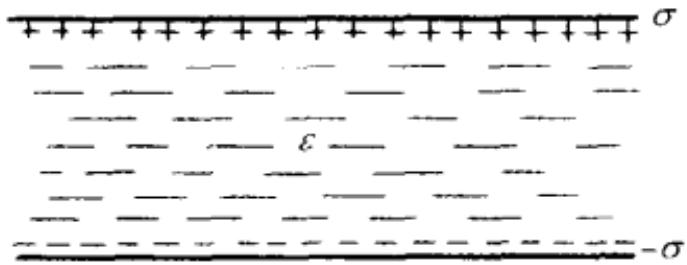
\includegraphics[width=0.5\linewidth]{figures/fig_2_2_3_1.jpg}
\end{center}
\begin{center}
    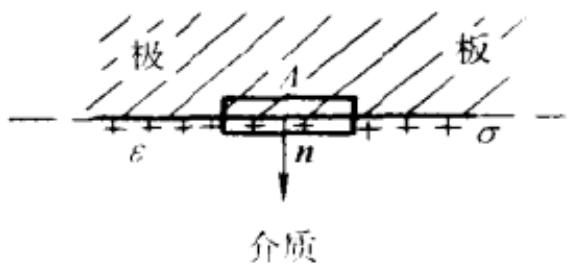
\includegraphics[width=0.5\linewidth]{figures/fig_2_2_3_2.jpg}
\end{center}

\vfill

\textbf{2.2.4.} 一平行板电容器两极板相距为 $2.0\mathrm{mm}$ ，电势差为 $400\mathrm{V}$ ，两极板间是介电常数为 $\varepsilon_{\mathrm{r}} = 5.0$ 的均匀玻璃片。略去边缘效应，试求玻璃表面上极化电荷量的面密度。

\vfill

\newpage

\textbf{2.2.5.} 一平行板电容器由面积都是 $50\mathrm{cm}^2$ 的两金属薄片贴在石蜡纸上构成，已知石蜡纸厚为 $0.10\mathrm{mm}$ ，介电常数为2.0。略去边缘效应，试问这电容器加上 $100\mathrm{V}$ 的电压时，每个极板上的电荷量是多少？

\vfill

\textbf{2.2.6.} 在静电场中,导体处在介质里. 试证明:(1)导体表面上电荷量的面密度 $\sigma$ 与该处介质中的电位移 $D$ 的关系为 $\sigma = n \cdot D$ , 式中 $n$ 是导体表面在该处外法线方向上的单位矢量;(2)该处介质表面上极化电荷量的面密度为 $\sigma' = -\left(1 - \frac{1}{\varepsilon_r}\right)\sigma$ , 式中 $\varepsilon_r$ 是介质的介电常数.

图2.2.6
\begin{center}
    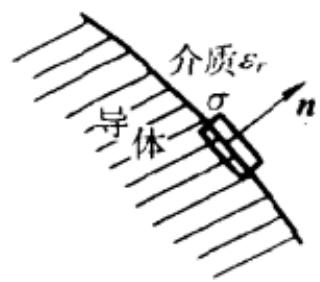
\includegraphics[width=0.5\linewidth]{figures/fig_2_2_6.jpg}
\end{center}

\vfill

\newpage

\textbf{2.2.7.} 一平行板电容器两极板相距为 d，接到电压为 U 的电源上，在其间插入厚为 t、介电常数为 $\varepsilon_{r}$ 的玻璃平板，如图 2.2.7 所示。略去边缘效应，试求空隙中和玻璃中的电场强度。
\begin{center}
    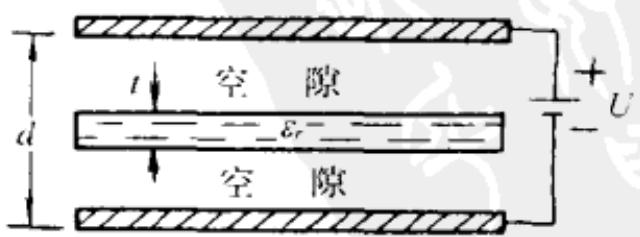
\includegraphics[width=0.5\linewidth]{figures/fig_2_2_7.jpg}
\end{center}

\vfill

\textbf{2.2.8.} 用两片面积都是 A 的金属片夹住两层均匀介质, 它们的厚度分别为 $d_{1}$ 和 $d_{2}$ , 电容率分别为 $\varepsilon_{1}$ 和 $\varepsilon_{2}$ , 如图 2.2.8 所示. 设两金属片上所带电荷量分别为 Q 和 -Q, 略去边缘效应, 试求两介质表面上极化电荷量的面密度和两金属片的电势差.

图2.2.8
\begin{center}
    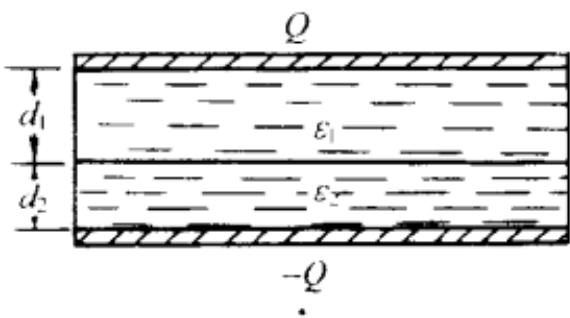
\includegraphics[width=0.5\linewidth]{figures/fig_2_2_8.jpg}
\end{center}

\vfill

\newpage

\textbf{2.2.9.} 两平行金属片相距为 $5.0\mathrm{mm}$ ，带有等量异号电荷，电荷量的面密度大小为 $20\mu \mathrm{C} / \mathrm{m}^2$ ；两片间有两层均匀介质，介电常数分别为 $\varepsilon_{\mathrm{r1}} = 3.0$ 和 $\varepsilon_{\mathrm{r2}} = 4.0$ 。略去边缘效应，试求各介质内的电场强度、电位移和介质表面上极化电荷量的面密度。

\vfill

\textbf{2.2.10.} 一平行板电容器两极板的面积都是 $2.0\mathrm{m}^2$ ，相距为 $5.0\mathrm{mm}$ ，两板加上10000伏特电压后，断开电源，再在其间充满两层均匀介质，一层厚 $2.0\mathrm{mm}$ ，介电常数为5.0；另一层厚 $3.0\mathrm{mm}$ ，介电常数为2.0。略去边缘效应。（1）试求各介质中极化强度的大小；(2)若与介电常数为2.0接触的极板接地（即电势为零），另一极板（正极板）的电势是多少？两介质接触面上的电势是多少？

\vfill

\newpage

\textbf{2.2.11.} 两块相同的平行金属片, 相距为 $d = 1.0 \mathrm{~cm}$ , 每片的面积都是 $200 \mathrm{~cm}^{2}$ , 两片间有一块面积相同的、厚为 $t = 5.0 \mathrm{~mm}$ 的平行石蜡板, 如图 2.2.11 (1) 所示. 给一金属片带上电荷量 $Q_{1} = 1.2 \times 10^{-10} \mathrm{C}$ , 另一金属片带上电荷量 $Q_{2} = 2.4 \times 10^{-10} \mathrm{C}$ . 已知石蜡的介电常数为 $\varepsilon_{\mathrm{r}} = 2.0$ . 略去边缘效应. 试求: (1) 金属片上电荷量的面密度; (2) 石蜡内的电场强度; (3) 两金属片的电势差; (4) 石蜡板表面极化电荷量的面密度.

图2.2.11(1)

图2.2.11(2)
\begin{center}
    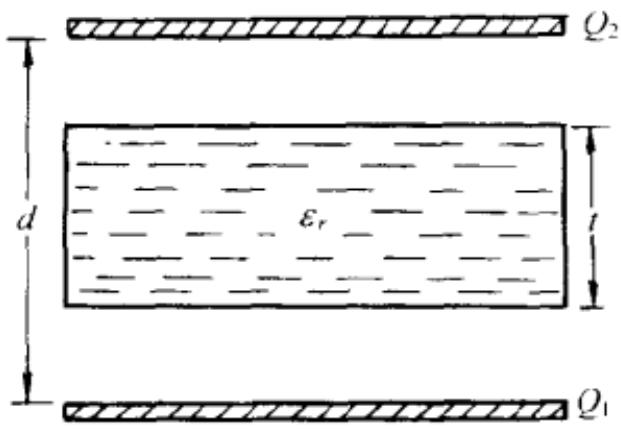
\includegraphics[width=0.5\linewidth]{figures/fig_2_2_11_1.jpg}
\end{center}
\begin{center}
    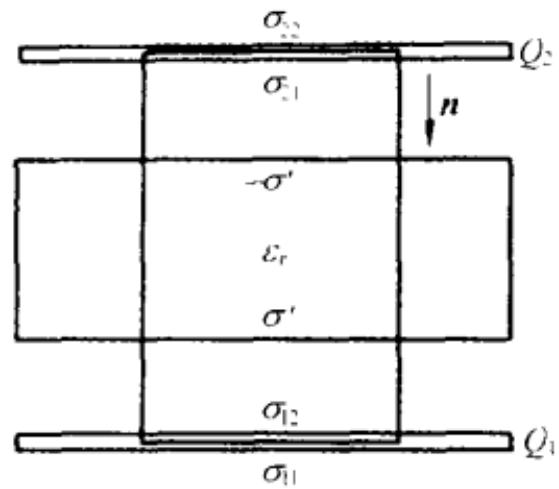
\includegraphics[width=0.5\linewidth]{figures/fig_2_2_11_2.jpg}
\end{center}

\vfill

\textbf{2.2.12.} 平行板电容器两极板 A、B 相距为 3.0cm，两板间有一层 $\varepsilon_{r}=2.0$ 的均匀介质，其位置和厚度如图 2.2.12(1) 所示。两极板带有等量异号电荷，电荷量的面密度大小为 $\sigma=8.9\times10^{-10}C/m^{2}$ 。略去边缘效应。（1）试求两极板间各处 E、D 和 P 的值以及极板间各处的电势（设 A 板电势为零）；（2）画出 E-x、D-x 和 U-x 曲线。
\begin{center}
    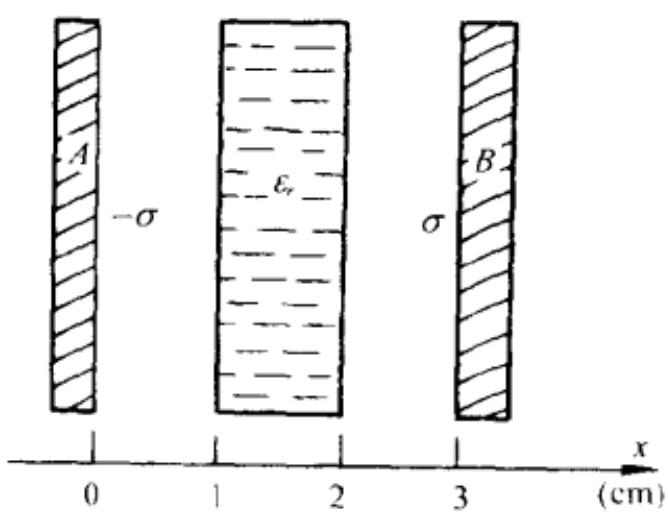
\includegraphics[width=0.5\linewidth]{figures/fig_2_2_12.jpg}
\end{center}

\vfill

\newpage

\textbf{2.2.13.} 平行板电容器两极板相距为 d，电势差为 U，其中有一层厚为 t 的均匀介质平行板，介电常数为 $\varepsilon_{r}$ ，介质两边都是空气，如图 2.2.13 所示。略去边缘效应。试求：(1) 介质中的电场强度、电位移和极化强度；

图2.2.13

(2)极板与介质间的电场强度和电位移；(3)极板上电荷

量的面密度 $\sigma$ ; 介质表面极化电荷量的面密度 $\sigma'$ .

\vfill

\textbf{2.2.14.} 一平行板电容器两极板间左半边是空气, 右半边是 $\varepsilon_{\mathrm{r}} = 3.0$ 的均匀介质, 如图 2.2.14 所示. 两极板相距为 $10 \mathrm{~mm}$ , 电势差为 $100 \mathrm{~V}$ . 略去边缘效应. 试分别求两极板间空气中和介质中的电场强度、电位移和极化强度的值.

图2.2.14
\begin{center}
    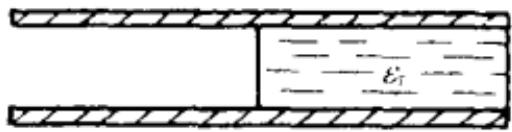
\includegraphics[width=0.5\linewidth]{figures/fig_2_2_14.jpg}
\end{center}

\vfill

\newpage

\textbf{2.2.15.} 将平行板电容器两极板接到电压为 U 的电源上(接通 K)，然后在两极板间的一半放入电容率为 $\varepsilon$ 的均匀介质，如图 2.2.15 所示。略去边缘效应。(1)试问 A、B 两点的电场强度哪个大？各为未放入介质时的多少倍？

(2)如果在充电后,先将电源断开,再在两极板间的一半放入介质,则结果如何?

\vfill

\textbf{2.2.16.} 在 $100^{\circ}C$ 和 $1.0atm$ 时，饱和水蒸气的密度为 $598g/m^{3}$ . 水的分子量为 18, 水分子的电偶极矩为 $6.2 \times 10^{-30}C \cdot m$ . 试求这时水蒸气的极化强度的最大值.

\vfill

\newpage

\textbf{2.2.17.} 一均匀介质球在均匀极化后,极化强度为 P. 试求:(1)它表面上极化电荷量的面密度;(2)这极化面电荷在球心产生的电场强度.

\vfill

\textbf{2.2.18.} 在 $\varepsilon_{r}=6.0$ 的瓷体表面附近, 空气里的电场强度 E 的大小为 $6.0\times10^{4}V/m$ , E 的方向与瓷体表面的外法线成 $45^{\circ}$ 角, 试求该处瓷体内电位移 D 的大小和方向以及瓷体表面上极化电荷量的面密度 $\sigma'$ .

图2.2.18
\begin{center}
    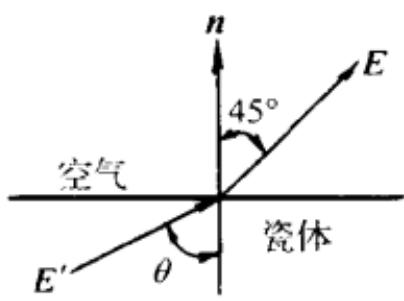
\includegraphics[width=0.5\linewidth]{figures/fig_2_2_18.jpg}
\end{center}

\vfill

\newpage

\textbf{2.2.19.} 两块平行金属板间充满电容率为 $\varepsilon_{1}$ 的均匀介质，在这介质内有一个电容率为 $\varepsilon_{2}$ 的均匀介质球。当两金属板加上电压后，两种情况下的电位移线分别如图2.2.19的(1)和(2)所示。试判定各图中 $\varepsilon_{1}$ 和 $\varepsilon_{2}$ 哪个大。


图2.2.19
(2)
\begin{center}
    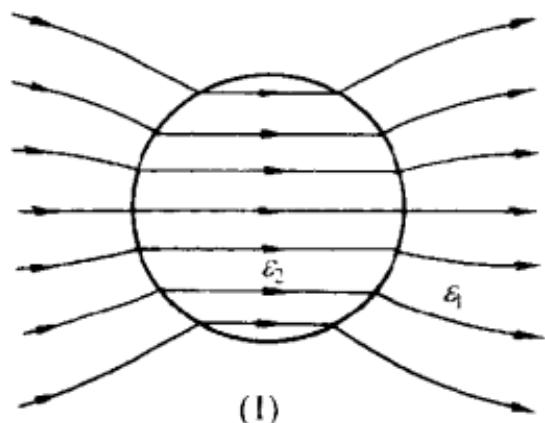
\includegraphics[width=0.5\linewidth]{figures/fig_2_2_19_1.jpg}
\end{center}
\begin{center}
    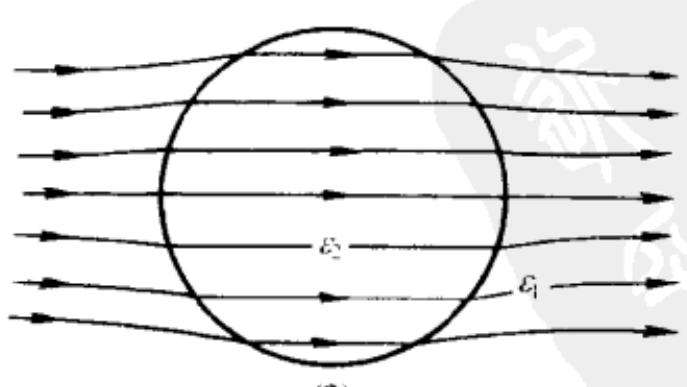
\includegraphics[width=0.5\linewidth]{figures/fig_2_2_19_2.jpg}
\end{center}

\vfill

\textbf{2.2.20.} 两介质的电容率分别为 $\varepsilon_{1}$ 和 $\varepsilon_{2}$ , 在它们的交界面上有一层电荷量的面密度为 $\sigma$ 的自由电荷; 这面两边的电场强度分别为 $E_{1}$ 和 $E_{2}$ , 它们与交界面法线的夹角分别为 $\theta_{1}$ 和 $\theta_{2}$ , 如图 2.2.20 所示. 试证明: $\varepsilon_{2} \cot \theta_{2} = \varepsilon_{1} \cot \theta_{1} \left(1 + \frac{\sigma}{\varepsilon_{1} E_{1} \cos \theta_{1}}\right)$ .

\vfill

\newpage

\textbf{2.2.21.} 在有介质时,高斯定理为 $\oiint_{S} D \cdot dS = Q$ , 式中 Q 是高斯面 S 内自由电荷量的代数和. 如果把介质都去掉, 而让自由电荷的分布和数量都保持原样, 这时便有 $\varepsilon_0\oiint_{S}\pmb {E}_0\cdot \mathrm{d}\pmb {S} = Q.$ (1)有人据此得出结论： $\pmb{D}$ 只由自由电荷决定，而与介

图2.2.21

质无关；D 等于介质不存在时的电场强度 $E_{0}$ 乘以 $\varepsilon_{0}$ . 你认为他这两个结论是否正确？为什么？(2) 假定均匀介质充满一半空间，另一半是真空，介质与真空的交界面是平面，在介质外面的真空中，有一个电荷量为 q 的点电荷，如图 2.2.21 所示．试将交界面两边的 D 与介质不存在

时这电荷产生的 $\varepsilon_{0}E_{0}$ 作比较,再评价上述结论.
\begin{center}
    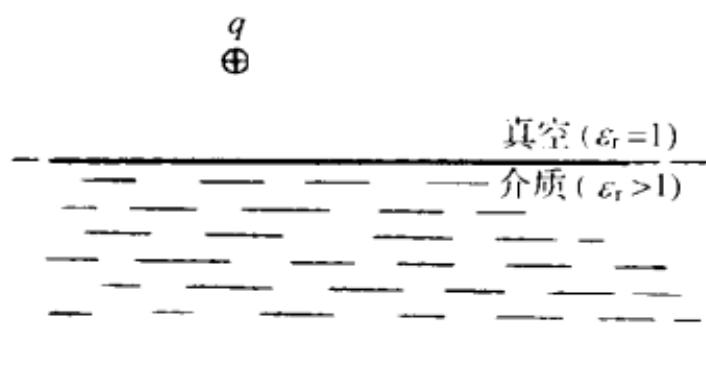
\includegraphics[width=0.5\linewidth]{figures/fig_2_2_21.jpg}
\end{center}

\vfill

\textbf{2.2.22.} 设极化电荷产生的电场强度为 $E'$ ，则在介质中取高斯面 $S$ ，便有 $\oiint_{S} E' \cdot \mathrm{d}S = \frac{1}{\varepsilon_0} q'$ ，式中 $q'$ 是 $S$ 所包住的极化电荷量的代数和。又由极化电荷量密度 $\rho'$ 与极化强度的关系 $\rho' = -\nabla \cdot P$ 得： $q' = \int_V \rho' \mathrm{d}V = \int_V (-\nabla \cdot P) \mathrm{d}V = -\oiint_{S} P \cdot \mathrm{d}S$ 。于是有 $\oiint_{S} \varepsilon_0 E' \cdot \mathrm{d}S = -\oiint_{S} P \cdot \mathrm{d}S$ 。由此得出： $\varepsilon_0 E' = -P$ 。这个结果对吗？为什么？

【解答】 不对. 由

$$
\oiint_ {S} \varepsilon_ {0} \boldsymbol {E} ^ {\prime} \cdot \mathrm{d} \boldsymbol {S} = - \oiint_ {S} \boldsymbol {P} \cdot \mathrm{d} \boldsymbol {S}
$$

可以得出

$$
\oiint_ {S} \left(\varepsilon_ {0} \boldsymbol {E} ^ {\prime} + \boldsymbol {P}\right) \cdot \mathrm{d} \boldsymbol {S} = 0
$$

但不能由此得出 $\varepsilon_0E' = -P$ 的结论. 因为一个矢量场对封闭曲面的积分为零, 不能得出该矢量场处处为零的结论.

\vfill

\newpage

\textbf{2.2.23.} 试证明下述两条关于静电场的定理:(1)凡是没有电荷的地方,该点的电势既不可能是极大值也不可能是极小值.换句话说,电势的极值只能出现在有电荷的地方;(2)凡是电势有极大值的地方,该点必定有正电荷;凡是电势有极小值的地方,该点必定有负电荷.

\vfill

\textbf{2.2.24.} 一无限大的均匀介质平板，厚为 $d$ ，电容率为 $\varepsilon$ ，其中分布着电荷量密度为 $\rho$ 的均匀自由电荷．试求板内外的电场强度 $E$ 、电位移 $D$ 、极化强度 $P$ 、极化电荷量密度 $\rho^{\prime}$ 和极化电荷量的面密度 $\sigma^{\prime}$ 等.

\vfill

\newpage

\textbf{2.2.25.} 一块硫磺平板, $\varepsilon_{r}=4.0$ ,放在均匀外电场中被均匀极化,板面的法线与外电场的方向平行. 已知它的表面上极化电荷量的面密度为 $5.0\mu \mathrm{C} / \mathrm{m}^2$ . 试求它里面的极化强度、电场强度、电位移等的值和它外面靠近板面处的电场强度和电位移的值.

\vfill

\textbf{2.2.26.} 一无限大的均匀介质平板,电容率为 $\varepsilon$ . 放在电场强度为 $E_0$ 的均匀外电场中,板面法线与 $E_0$ 成 $\theta$ 角. 试求板面上极化电荷量的面密度.

图2.2.26
\begin{center}
    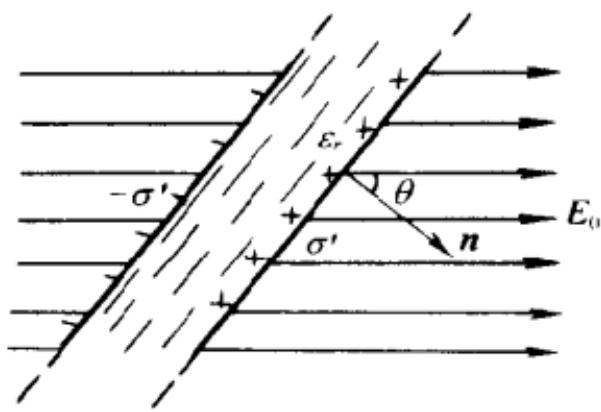
\includegraphics[width=0.5\linewidth]{figures/fig_2_2_26.jpg}
\end{center}

\vfill

\newpage

\textbf{2.2.27.} 一细长的均匀圆柱体,电容率为 $\varepsilon$ ,放在电场强度为 $E_0$ 的均匀外电场中,被均匀极化,柱体的轴线与 $E_0$ 平行.试求圆柱体中心 $C$ 处的电场强度 $E_C$ 和电位移 $D_C$ 以及表面上的极化电荷量的面密度 $\sigma'$ .

\vfill

\textbf{2.2.28.} 将一个介电常数为 $\varepsilon_{\mathrm{r}}$ 的均匀介质球，放在电场强度为 $E_0$ 的均匀外电场中，被均匀极化。试求球的极化强度 $P$ 和球心的电场强度 $E_C$ 。

\vfill

\newpage

\textbf{2.2.29.} 在介电常数为 $\varepsilon_{\mathrm{r}} = 3.0$ 的均匀介质内存在电场强度为 $E_0 = 2.0 \times 10^{6} \mathrm{~V} / \mathrm{m}$ 的均匀电场，这介质内有一扁鼓形空穴，其两底面与 $E_0$ 垂直。试求这空穴中心的电场强度 $E_C$ 和两底面上极化电荷量的面密度 $\sigma'$ 。

\vfill

\textbf{2.2.30.} 在介电常数为 $\varepsilon_{\mathrm{r}} = 5.0$ 的均匀介质内，有两个相距很远的空穴，一个是薄扁鼓形，两底面垂直于介质内的电位移 $D$ ；另一个是细长圆柱形，轴线平行于 $D$ 。空穴内都是空气。已知 $D$ 的值为 $D = 1.0 \times 10^{-8} \mathrm{C} / \mathrm{m}^2$ 。试求两空穴中心电场强度 $E$ 的值。

\vfill

\newpage

\textbf{2.2.31.} 一半径为 $a$ 的金属球外有一同心的金属球壳，壳的内半径为 $b$ ，球与壳间充满一种球对称的介质，它的电容率与到球心距离 $r$ 的 $n$ 次方成正比，即 $\varepsilon \propto r^n$ ，如图2.2.31所示．已知球的电势为 $U_{a}$ ，壳的电势为 $U_{b}$ ．试证明：在球与壳间离球心为 $r$ 处的电势为


$$
U _ {r} = \frac {a ^ {n + 1} U _ {a} - b ^ {n + 1} U _ {b}}{a ^ {n + 1} - b ^ {n + 1}} - \frac {U _ {a} - U _ {b}}{a ^ {n + 1} - b ^ {n + 1}} \left(\frac {a b}{r}\right) ^ {n + 1}
$$

图2.2.31
\begin{center}
    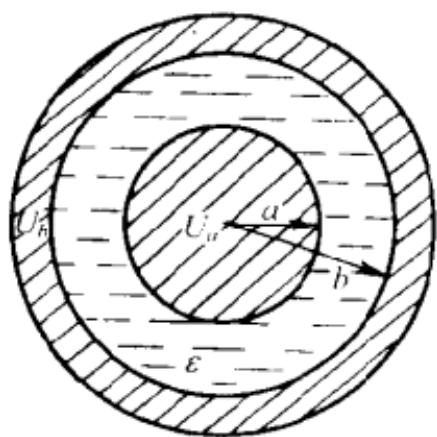
\includegraphics[width=0.5\linewidth]{figures/fig_2_2_31.jpg}
\end{center}

\vfill

\textbf{2.2.32.} 一金属球带有电荷量 $Q$ ，球外有一内半径为 $b$ 的金属球壳，球壳接地，球与壳间充满介质，其介电常数与到球心的距离 $r$ 的关系为 $\varepsilon_{\mathrm{r}} = \frac{c + r}{r}$ ，式中 $c$ 是常数。以地的电势为零。试证明：离球心为 $r$ 处的电势为

$$
U _ {r} = \frac {Q}{4 \pi \varepsilon_ {0} c} \ln \frac {b (r + c)}{(b + c) r}
$$

\vfill

\newpage

\textbf{2.2.33.} 半径为 $R$ 、电容率为 $\varepsilon$ 的均匀介质球中心，放有电荷量为 $Q$ 的点电荷，球外是空气。（1)试求球内外的电场强度 $\pmb{E}$ 和电势 $U$ ；（2）如果要使球外的电场强度为零而球内的电场强度不变，则球面上应放的电荷量为多少？这电荷量如何分布？

\vfill

\textbf{2.2.34.} 半径为 $R$ 的金属球带有电荷量 $Q$ , 处在电容率为 $\varepsilon$ 的无限大均匀介质中. 试求介质内离球心为 $r$ 处的电场强度 $E$ 、电位移 $D$ 、极化强度 $P$ 、极化电荷量密度 $\rho'$ 和介质表面上极化电荷量的面密度 $\sigma'$ .

\vfill

\newpage

\textbf{2.2.35.} 半径为 R 的金属球带有电荷量 Q，球外有一同心的介质球壳，其内外半径分别为 a 和 b，电容率为 $\varepsilon$ ，如图 2.2.35 所示。试求：(1) 各处的电场强度 E 和电位移 D；(2) 介质的极化强度 P 和极化电荷量密度 $\rho'$ 以及表面上极化电荷量的面密度 $\sigma'$ ；(3) 各处的电势 U。

\vfill

\textbf{2.2.36.} 半径为 R 的金属球外包着一层厚为 R 的介质球壳, 壳的介电常数为 $\varepsilon_{r}=2$ , 壳外是真空, 如图 2.2.36 所示. 现将电荷量为 Q 的自由电荷均匀分布在介质壳体内. 在金属球的电势为零的情况下, 试求介质壳的外表面上的电势.

\vfill

\newpage

\textbf{2.2.37.} 电介质强度是指电介质能经受的最大电场强度而不被击穿,迄今所知道的电介质强度的最大值约为 $1 \times 10^{9} \mathrm{~V} / \mathrm{m}$ , 介电常数约为 2. 当金属处在这种介质中时,试问: (1) 它的表面上电荷量的面密度最大不能超过多少? (2) 该金属原子的直径约为 $2 \times 10^{-10} \mathrm{~m}$ , 它表面一层原子中, 缺少或多出一个电子的原子数, 最多不超过百分之几?

【解答】（1）电荷量的面密度的最大值为

$$
\begin{array}{r l} \sigma_ {\max} & = D _ {\max} = \epsilon_ {r} \varepsilon_ {0} E _ {\max} = 2 \times 8. 8 5 4 \times 1 0 ^ {- 1 2} \times 1 \times 1 0 ^ {9} \\ & = 1. 8 \times 1 0 ^ {- 2} (\mathrm {C/ m^ {2}}) \end{array}\tag{1}
$$

(2)设原子的直径为 $d$ ，电子电荷的大小为 $\pmb{e}$ ，则该金属表面单位面积上最多缺少或多出的电子数为

$$
n _ {\max} = \frac {\sigma_ {\max}}{e} = \frac {\varepsilon_ {r} \varepsilon_ {0} E _ {\max}}{e}\tag{2}
$$

单位面积上表面一层的原子数为

$$
N = \frac {1}{d ^ {2}}\tag{3}
$$

故该金属带电时，表面一层原子中缺少或多出一个电子的原子数所占的百分比最多为

$$
\begin{aligned} \frac{n_{\max}}{N} & = \frac{\varepsilon_{\mathrm{r}}\varepsilon_{0}E_{\max}d^{2}}{e}\\ & = \frac{2\times 8.854\times 10^{-12}\times 1\times 10^{9}\times(2\times 10^{-10})^{2}}{1.6\times 10^{-19}}\\ & = 4\times 10^{-3} = 0.4\% \end{aligned}\tag{4}
$$

\vfill

\textbf{2.2.38.} 空气的电介质强度为 $E_{m}=3000kV/m$ ，问直径为 1.0cm 和 1.0mm 的金属球，在空气中最多能带多少电荷量？

\vfill

\newpage

\textbf{2.2.39.} 空气的电介质强度为 $3000 \, kV/m$ ，铜的密度为 $8.9 \, g/cm^{3}$ ，铜的原子量为每摩尔 63.75 克，阿伏伽德罗常量为 $6.022 \times 10^{23} (\text{mol})^{-1}$ ，金属铜里每个铜原子有一个自由电子，每个电子电荷量的大小为 $1.60 \times 10^{-19} C$ 。(1)试问半径为 1.0 厘米的铜球在空气中最多能带多少电荷量？(2)这铜球带电最多时，试求它所缺少或多出的电子数与自由电子总数之比；(3)因导体球带电时电荷都在表面上，当铜球带电最多时，试求它所缺少或多出的电子数与表面一层铜原子所具有的自由电子数之比。

\vfill

\textbf{2.2.40.} 空气的电介质强度为 $3.0 \times 10^{6} ~V/m$ 。试问空气中半径为 $20 ~cm$ 的金属球，最高能维持多高的电势？某范德格拉夫起电机上金属球壳的外直径为 $1.0 ~m$ ，壳外是空气，试问它的电势最高能达到多少？

\vfill

\newpage

\textbf{2.2.41.} 用细玻璃管吹肥皂泡, 如果停止吹气并让玻璃管直通大气, 则由于表面张力, 肥皂泡将会收缩而消失. 现在让这肥皂泡带电, 使它不致收缩(图2.2.41). (1)试证明: 肥皂泡要维持半径为 $R$ 所需的电荷量为 $Q = \sqrt{128\pi^2\varepsilon_0\alpha R^3}$ , 式中 $\alpha$ 是肥皂水的表面张力系数; (2)当 $\alpha = 5.0\times 10^{-2}\mathrm{N / m}, R = 1.0\mathrm{cm}$ 时, 求 $Q$ 的值; (3)试证明: 设空气的电介质强度为 $E_{m}$ , 则当 $R < \frac{8\alpha}{\varepsilon_0E_m^2}$ 时, 就不可能用带电的方法维持肥皂泡而不使它消失; (4)设 $E_{m} = 3.0\times 10^{6}\mathrm{V / m}$ , 试计算用带电的方法能维持肥皂泡的半径 $R$ 的极小值.

图2.2.41
\begin{center}
    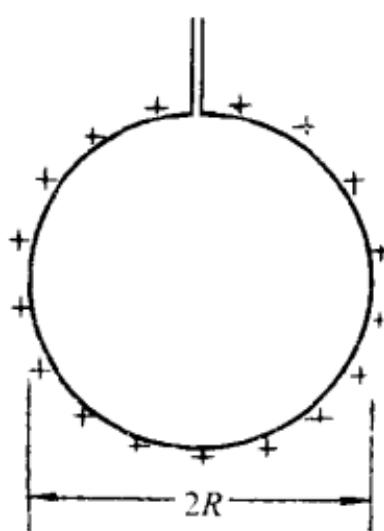
\includegraphics[width=0.5\linewidth]{figures/fig_2_2_41.jpg}
\end{center}

\vfill

\textbf{2.2.42.} 空气的电介质强度为 $E_{m}=3000kV/m$ ，试问空气中半径为 1.0cm、1.0mm 和 0.10mm 的长直导线上单位长度最多各能带多少电荷量？

\vfill

\newpage

\textbf{2.2.43.} 一盖革-米勒计数管，由直径为 $0.2\mathrm{mm}$ 的长直金属丝和套在它外面的同轴金属圆筒构成，圆筒的直径为 $20\mathrm{mm}$ ，金属丝与圆筒间充以氩气和乙醇蒸气，其电介质强度为 $4.3 \times 10^{6}\mathrm{V / m}$ . 略去边缘效应，试问金属丝与圆筒间的电压最大不能超过多少？

\vfill

\textbf{2.3.1.} 平行板电容器的两个极板 A 和 B 都是金属片, 充电时, 把 A 板接到电源正极, B 板接到电源负极; 充电后, 断开电源. 这时 A、B 两板外的电荷和电力线, 有人画成图 2.3.1(1) 的样子, 也有人画成图 2.3.1(2) 的样子. 你认为哪个对? 为什么?

(1)

(2)
图2.3.1

【解答】因为 A 板曾接过电源正极，B 板曾接过电源负极，故 A 板带正电，B 板带负电，A 板电势高于 B 板；电源断开后，仍然如此。根据电势差的定义得

$$
U _ {A} - U _ {B} = \int_ {A} ^ {B} \boldsymbol {E} \cdot \mathrm{d} l > 0\tag{1}
$$

因电力线是从高电势走向低电势,故沿着它的箭头方向走,电势便越来越低.若按图2.3.1(1)的极板外那条电力线从A到B积分,则有

$$
\int_ {A} ^ {B} \boldsymbol {E} \cdot \mathrm{d} \boldsymbol {l} = \int_ {A} ^ {B} E \cos 0 \mathrm{d} l = \int_ {A} ^ {B} E \mathrm{d} l > 0\tag{2}
$$

结果得 $U_{A} > U_{B}$ 这是对的. 若按图2.3.1(2)的极板外那条电力线积分, 则有

$$
\int_ {A} ^ {B} \boldsymbol {E} \cdot \mathrm{d} \boldsymbol {l} = \int_ {A} ^ {B} E \cos \pi \mathrm{d} l = - \int_ {A} ^ {B} E \mathrm{d} l <   0\tag{3}
$$

结果得 $U_{A} < U_{B}$ . 这显然不对. 因此, 对 $A, B$ 两极板外的电力线来说, 图2.3.1(1)是对的, 而图2.3.1(2)则是错的.
\begin{center}
    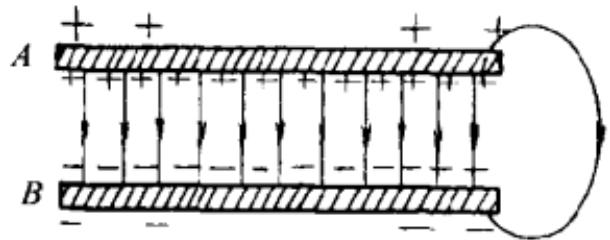
\includegraphics[width=0.5\linewidth]{figures/fig_2_3_1_1.jpg}
\end{center}
\begin{center}
    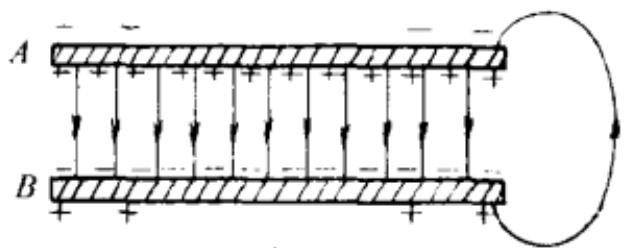
\includegraphics[width=0.5\linewidth]{figures/fig_2_3_1_2.jpg}
\end{center}

\vfill

\newpage

\textbf{2.3.2.} 一平行板电容器的两极板相距为 $1.0\mathrm{mm}$ ，两极板都是正方形，面积相等，两板间是空气。当它的电容为(1) $1.0\mathrm{F}$ ，(2) $10\mu \mathrm{F}$ 和(3) $100\mathrm{pF}$ 时，略去边缘效

应,试求相应的边长.

\vfill

\textbf{2.3.3.} 面积都是 $2.0 ~m^{2}$ 的两平行金属片放在空气中相距 5.0 mm，两片的电势差为 1000 V。略去边缘效应，试求：(1) 电容 C；(2) 各片上的电荷量 Q 和电荷量的面密度 $\sigma$ ；(3) 两片间电场强度 E 的值。

\vfill

\newpage

\textbf{2.3.4.} 电容器由三片面积都是 $6.0 \, cm^{2}$ 的锡箔构成，相邻两箔间的距离都是 0.10 mm，外边两片联在一起成为一极，中间一片作为另一极，如图

\vfill

\textbf{2.3.4.} 所示. 略去边缘效应. (1) 试求电容 C; (2) 若在这电容器两极加上 220 伏的

电压,问三箔上电荷量的面密度各是多少?

\vfill

\newpage

\textbf{2.3.5.} 11 张金属箔平行排列, 奇数箔联在一起作为电容器的一极, 偶数箔联在一起作为另一极, 如图 2.3.5 所示, 已知每张箔的面积都是 $1.0 \mathrm{~m}^{2}$ , 相邻两箔间的距离都是 $5.0 \mathrm{~mm}$ , 箔间都是空气. 略去边缘效应. 试求电容 C.

图2.3.5
\begin{center}
    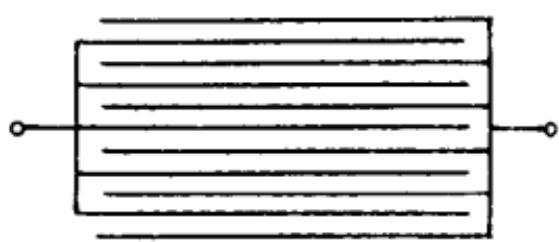
\includegraphics[width=0.5\linewidth]{figures/fig_2_3_5.jpg}
\end{center}

\vfill

\textbf{2.3.6.} 一云母电容器由10张铝箔和9片云母片相间平行叠放而成，奇数铝箔接在一起作为一极，偶数铝箔接在一起作为另一极，如图2.3.6所示。每张铝箔和每片云母的面积都是 $2.5cm^{2}$ ，每片云母片的介电常数都是7.0，厚度都是0.15mm。略去边缘效应，试求电容C。

\vfill

\newpage

\textbf{2.3.7.} 平行板电容器两极板的面积都是 S，相距为 d，其间有一厚为 t 的平行金属片，如图 2.3.7 所示。略去边缘效应。（1）试求电容 C；（2）试问金属片离极板的远近有无影响？（3）当 $t \to 0$ 和 $t \to d$ 时 C 各为多少？
\begin{center}
    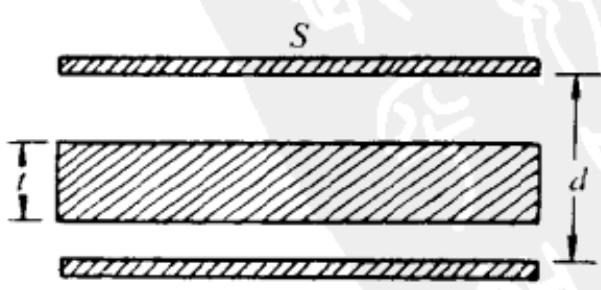
\includegraphics[width=0.5\linewidth]{figures/fig_2_3_7.jpg}
\end{center}

\vfill

\textbf{2.3.8.} 一平行板电容器的极板面积为 S，两极板相距为 d，其间有一层电容

图2.3.8

率为 $\varepsilon$ 、厚为 $t$ 的介质，如图2.3.8所示。略去边缘效应。（1）试求它的电容 $C$ ；（2）当 $S = 500\mathrm{mm} \times 500\mathrm{mm}, d = 10\mathrm{mm}, t = 6.0\mathrm{mm}, \varepsilon = 4.0\varepsilon_0$ 时，计算 $C$ 的值。
\begin{center}
    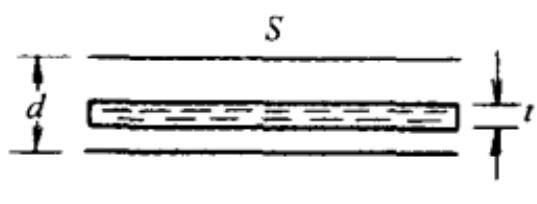
\includegraphics[width=0.5\linewidth]{figures/fig_2_3_8.jpg}
\end{center}

\vfill

\newpage

\textbf{2.3.9.} 一平行板电容器两极板的面积都是 $S = 100\mathrm{cm}^2$ ，相距为 $d = 1.0\mathrm{cm}$ 将两极板接到100伏的电源上充电后，断开电源，再在两极板间放入一层 $\varepsilon_r = 7.0$ 的电介质，其厚为 $t = 0.50\mathrm{cm}$ 略去边缘效应。试求：(1)未放入介质前的电容 $C_0$ ；(2)极板上的电荷量；(3)介质内外的电场强度；(4)放入介质后两极板的电势差；(5)放入介质后的电容 $C$ 。

\vfill

\textbf{2.3.10.} 一空气平行板电容器的电容为 $C_0 = 9.8\mathrm{pF}$ , 极板间的距离为 $d = 1.0\mathrm{cm}$ , 现将介电常数为 $\varepsilon_{\mathrm{r}} = 2.0$ 的橡皮膜平行地放在极板间, 如图2.3.10所示, 测得这时电容为 $C = 10$ 皮法. 略去边缘效应, 试求橡皮膜的厚度 $x$ .

\vfill

\newpage

\textbf{2.3.11.} 一平行板电容器两极板的面积均为 $S$ ，相距为 $d$ ，其间充满介质，介质的电容率是变化的，在一极板处为 $\varepsilon_1$ ，在另一极板处为 $\varepsilon_2$ ，其他处的电容率与到 $\varepsilon_1$ 处的距离成线性关系。略去边缘效应。（1）试求这电容器的电容，并检验你的结果在 $\varepsilon_2 = \varepsilon_1$ 时是否正确；（2）当两极板上的电荷量分别为 $Q$ 和 $-Q$ 时，试求介质内的极化电荷量密度 $\rho'$ 和表面上极化电荷量的面密度 $\sigma'$ 。

\vfill

\textbf{2.3.12.} 一平行板电容器两极板的面积都是 S，其间夹住两层电介质，厚度分别为 $d_{1}$ 和 $d_{2}$ ，电容率分别为

$\varepsilon_{1}$ 和 $\varepsilon_{2}$ , 如图2.3.12所示. 略去边缘效应. 试求这电容器的电容 $C$ , 并用 $\varepsilon_{2} = \varepsilon_{1}$ 检验一下你的结果.

\vfill

\newpage

\textbf{2.3.13.} 一平行板电容器两极板的面积都是 S，其间有 n 层平行介质层，它们的电容率分别为 $\varepsilon_{1}$ 、 $\varepsilon_{2}$ 、 $\cdots$ 、 $\varepsilon_{n}$ ，厚度分别为 $d_{1}$ 、 $d_{2}$ 、 $\cdots$ 、 $d_{n}$ ，如图 2.3.13 所示。略去边缘效应。试求这电容器的电容。

\vfill

\textbf{2.3.14.} 一平行板电容器两极板的面积都是 $200\mathrm{mm}^2$ ，两板间夹住一块两面都涂有石蜡的玻璃片，玻璃片厚为 $1.0\mathrm{mm}$ ，介电常数为 $\varepsilon_{r1} = 7.0$ ；两层石蜡的厚度都是 $0.2\mathrm{mm}$ ，介电常数为 $\varepsilon_{r2} = 2.0$ 略去边缘效应，试求这电容器的电容.

\vfill

\newpage

\textbf{2.3.15.} 一平行板电容器两极板的面积都是 $2.0\mathrm{m}^2$ ，相距为 $5.0\mathrm{mm}$ 。当两板之间是空气时，加上一万伏电压后，断开电源，再在其间插入两平行介质层，一层介电常数为5.0，厚为 $2.0\mathrm{mm}$ ；另一层介电常数为2.0，厚为 $3.0\mathrm{mm}$ 。略去边缘效应。试求：(1)介质中 $\pmb{E}$ 和 $\pmb{D}$ 的值；(2)两极板的电势差 $U$ ；(3)电容 $C$

\vfill

\textbf{2.3.16.} 一平行板电容器两极板相距为 $d$ ，其间充满了两部分均匀介质，电容率为 $\varepsilon_{1}$ 的介质所占的面积为 $S_{1}$ ，电容率为 $\varepsilon_{2}$ 的介质所占的面积为 $S_{2}$ ，如图2.3.16所示。略去边缘效应。试求这电容器的电容。

\vfill

\newpage

\textbf{2.3.17.} 一平行板电容器两极板的面积都是 $S$ ，相距为 $d$ ，今在其间平行地插入厚为 $t$ 、电容率为 $\varepsilon$ 的均匀介质片，其面积为 $S / 2$ ，如图2.3.17所示。设两极板分别带有电荷量 $Q$ 和 $-Q$ 。略去边缘效应。试求：(1)两极板的电势差；(2)电容 $C$ ；(3)介质片表面上极化电荷量的面密度。

\vfill

\textbf{2.3.18.} 电解质电容器有两个特点:一是电容 C 比较大;二是有正负极(在使用时不能接错).试说明它为什么有这两个特点.


【解答】电解质电容器(图2.3.18是电解质电容器的一种)是以金属作正极,在金属表面生成一层氧化膜(如图中的 $Al_{2}O_{3}$ )作为介质的电容器,其负极是非体电解质或固体电解质(如图中浸有电解质的衬垫纸).由于氧化膜极薄,介电常数又很大(如 $Al_{2}O_{3}$ 的 $\varepsilon_{r}=7$ 至10),所以电容就很大.

图2.3.18

图2.3.18 因为氧化膜具有单向导电性，电流只能从金属流向氧化膜；如果电流反向，氧化膜就会遭到破坏。因此电解质电容器就有正负极。
\begin{center}
    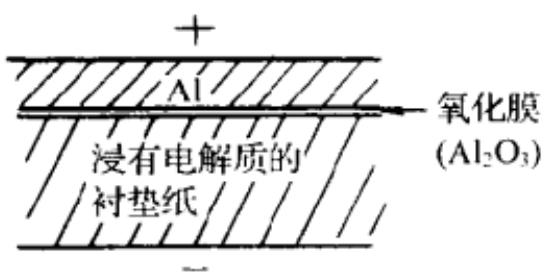
\includegraphics[width=0.5\linewidth]{figures/fig_2_3_18.jpg}
\end{center}

\vfill

\newpage

\textbf{2.3.19.} 收音机里用的一种可变电容器如图 2.3.19 所示, 其中共有 n 个面积均为 S 的金属片, 相邻两片的距离都是 d, 奇数片联在一起作为一极, 它固定不动(称为定片); 偶数片联在一起作为另一极, 它可以绕轴转动(称为动片). (1) 为什么动片转动时电容 C 会变? 转到什么位置时 C 最大? 转到什么位置时 C 最小? (2) 试证明: 略去边缘效应时, C 的最大值为 $C_{\max} = \frac{(n-1)\varepsilon_0 S}{d}$ .


图2.3.19
\begin{center}
    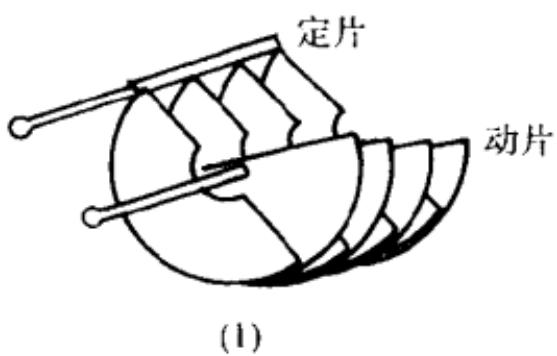
\includegraphics[width=0.5\linewidth]{figures/fig_2_3_19_1.jpg}
\end{center}
\begin{center}
    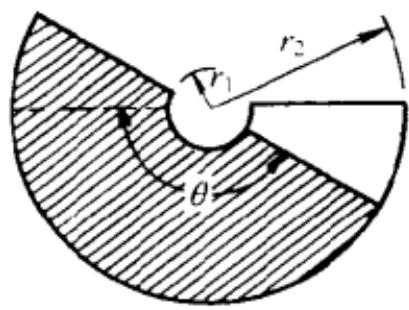
\includegraphics[width=0.5\linewidth]{figures/fig_2_3_19_2.jpg}
\end{center}

\vfill

\textbf{2.3.20.} 收音机里用的一种可变电容器如图 2.3.19 所示, 其中共有 n 个面积均为 S 的金属片, 相邻两片间的距离都是 d, 奇数片联在一起作为一极, 它固定不动(称为定片); 偶数片联在一起作为另一极, 它可以绕轴转动(称为动片). 当动片转到两组片之间夹角为 $\theta$ 时, 如图 2.3.19 的(2)所示, 试证明: 在 $\theta$ 较大的情况下, 略去边缘效应, 这电容器的电容为

$$
C = \frac {(n - 1) \pi \varepsilon_ {0} (r _ {2} ^ {2} - r _ {1} ^ {2}) \theta}{3 6 0 d}
$$

式中 $r_{1}$ 和 $r_{2}$ 分别为金属片内外缘的半径, $\theta$ 以度为单位.

\vfill

\newpage

\textbf{2.3.21.} 圆柱电容器由半径为 $a$ 的一段直导线和套在它外面的同轴导体圆筒构成, 圆筒的内半径为 $b$ , 导线与圆筒间是空气, 导线和圆筒的长度都是 $L$ . 略去边缘效应. 试求这电容器的电容.

\vfill

\textbf{2.3.22.} 试证明: 当圆柱电容器(见前面2.3.21题)两极的半径相差很小(即 $b - a \ll a$ )时, 它的电容 C 的公式趋于平行板电容器的公式.

\vfill

\newpage

\textbf{2.3.23.} 圆柱电容器是由半径为 $R_{1}$ 的直导线和与它同轴的导体圆筒构成，圆筒长为 $l$ ，内半径为 $R_{2}$ ，圆筒与导线间充满电容率为 $\varepsilon$ 的均匀介质，如图2.3.23所示.设导线上沿轴线单位长度的电荷量为 $\lambda$ ，圆筒上沿轴线单位长度的电荷量为-λ，略去边缘

效应,试求:(1)介质中的电场强度 E、电位移 D、极化强度 P、极化电荷量密度 $\rho'$ 和表面极化电荷量的面密度 $\sigma'$ ;(2)导线与圆筒的电势差 U;(3)电容 C.

\vfill

\textbf{2.3.24.} 一圆柱电容器由半径为 $a$ 的直导线和与它同轴的导体圆筒构成，圆筒的半径为 $b$ ，长为 $l$ ，导线与圆筒间充满了两层同轴圆筒形的均匀介质，交界面的半径为 $r$ ，电容率分别为 $\varepsilon_{1}$ （在内）和 $\varepsilon_{2}$ ，如图2.3.24所示。略去边缘效应，试求这电容器的电容。

图2.3.24
\begin{center}
    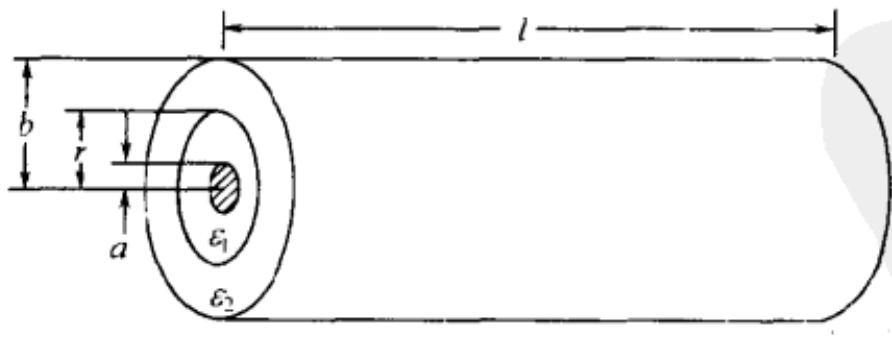
\includegraphics[width=0.5\linewidth]{figures/fig_2_3_24.jpg}
\end{center}

\vfill

\newpage

\textbf{2.3.25.} 三个共轴的金属圆筒, 长度都是 $l$ , 半径分别为 $a, b$ 和 $c$ , 它们的厚度都可略去不计, 如图 2.3.25 所示. 三圆筒间都是空气. 现将内外两圆筒联在一起作为电容器的一极, 中间圆筒作为另一极, 略去边缘效应. (1) 试求这电容器的电容 $C$ ; (2) 当 $l = 10 \mathrm{~cm}, a = 3.9 \mathrm{~mm}, b = 4.0 \mathrm{~mm}, c = 4.1 \mathrm{~mm}$ 时, 计算 $C$ 的值.

图2.3.25
\begin{center}
    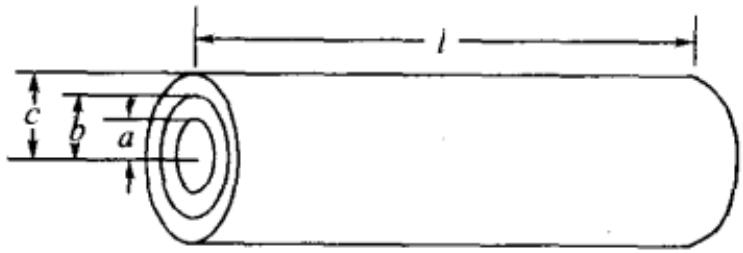
\includegraphics[width=0.5\linewidth]{figures/fig_2_3_25.jpg}
\end{center}

\vfill

\textbf{2.3.26.} 球形电容器是由两个同心的导体球壳构成,内壳的外半径为 a,外壳的内半径为 b,两壳间是空气.(1)试求这电容器的电容 C;(2)试证明:当两球壳相距很近(即 $b-a \ll a$ )时,C 趋于平行板电容器的电容公式;(3)试证明:当两球壳相距很远(即 $b \gg a$ )时,C 趋于一个孤立导体球的电容公式.

\vfill

\newpage

\textbf{2.3.27.} 一球形电容器由两个同心的薄导体球壳构成, 它们的半径分别为 $R_{1}$ 和 $R_{4}$ , 它们是电容器的两极, 在这两极之间有一个同心的不带电导体球壳, 其内外半径分别为 $R_{2}$ 和 $R_{3}$ , 如图 2.3.27 所示. (1) 给内壳 $(R_{1})$ 以电荷量 $Q$ , 求 $R_{1}$ 和 $R_{4}$ 两壳的电势差; (2) 求这电容器的电容.

\vfill

\textbf{2.3.28.} 一球形电容器由两个同心的薄金属球壳构成，两壳的半径分别为 $R_{1}$ 和 $R_{2}$ ，两壳间充满电容率为 $\varepsilon$ 的均匀介质，内壳带有电荷量 $Q$ ，如图2.3.28所示。试求：(1)两壳的电势差；(2)介质表面极化电荷量的面密度；(3)电容。

\vfill

\newpage

\textbf{2.3.29.} 一球形电容器由半径为 $R_{1}$ 的导体球和与它同心的导体球壳构成，壳的内半径为 $R_{2}$ ，球与壳间有一层同心的均匀介质球壳，其内外半径分别为 $a$ 和 $b$ ，电容率为 $\varepsilon$ ，如图2.3.29所示。（1）试求这电容器的电容；(2)当内球带有电荷量 $Q$ 时，介质内外表面上的极化电荷量的面密度各是多少？
\begin{center}
    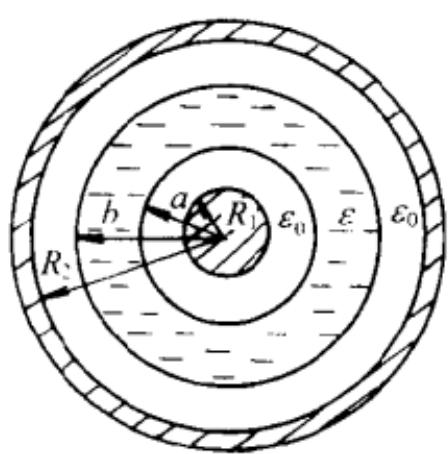
\includegraphics[width=0.5\linewidth]{figures/fig_2_3_29.jpg}
\end{center}

\vfill

\textbf{2.3.30.} 一球形电容器由半径为 $R_{1}$ 的导体球和与它同心的导体球壳构成, 壳的内半径为 $R_{2}$ , 球与壳间有两层均匀介质, 电容率分别为 $\varepsilon_{1}$ 和 $\varepsilon_{2}$ , 它们的交界面是半径为 $r$ 的同心球面, 如图 2.3.30 所示. (1) 试求这电容器的电容; (2) 当内球带有电荷量 $Q$ 时, 试求介质表面上极化电荷量的面密度.

\vfill

\newpage

\textbf{2.3.31.} 一球形电容器由半径为 $R_{1}$ 的导体球和与它同心的导体球壳构成, 壳的内半径为 $R_{2}$ , 球与壳间的一半充满电容率为 $\varepsilon$ 的均匀介质, 另一半是空气, 如图 2.3.31 所示. 试求这电容器的电容.

\vfill

\textbf{2.3.32.} 一同心球电容器由两个同心的导体球壳构成,两壳间一半充满电容率为 $\varepsilon$ 的均匀介质,另一半是空气,如图2.3.32所示.试证明,这电容器的电容等于两壳间充满电容率为 $\frac{\varepsilon + \varepsilon_0}{2}$ 的均匀介质的电容.

\vfill

\newpage

\textbf{2.3.33.} 空气中半径分别为 $a$ 和 $b$ 的两个金属球, 球心相距为 $d$ , 在 $d$ 比 $a$ 和 $b$ 都大相当多的情况下, 可以这样来估算它们之间的电容: 把两个球上的电荷在球外产生的电场, 近似地当作每个球上的电荷都集中在各自的球心时所产生的电场. (1) 试估算两球间的电容; (2) 当 $d \gg a$ 和 $b$ 时, $C$ 的值如何?

图2.3.33
\begin{center}
    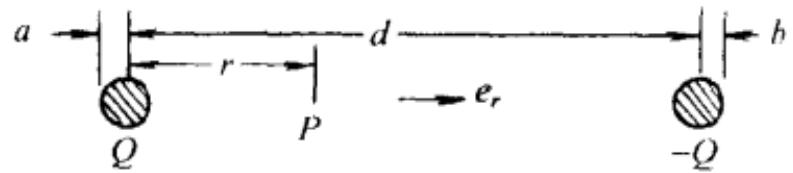
\includegraphics[width=0.5\linewidth]{figures/fig_2_3_33.jpg}
\end{center}

\vfill

\textbf{2.3.34.} 一个导体球(孤立导体球)的电容是指它所带的电荷量与它的电势(以无穷远处电势为零)的比值。(1)试求半径为 R 的孤立导体球的电容;(2)地球的半径为 6370 公里,把地球当作真空中的孤立导体球,试计算它的电容的值.

\vfill

\newpage

\textbf{2.3.35.} 半径都是 $a$ 的两根平行长直导线, 中心相距为 $d$ , 已知 $d \gg a$ . 试求它们间单位长度的电容.

图2.3.35
\begin{center}
    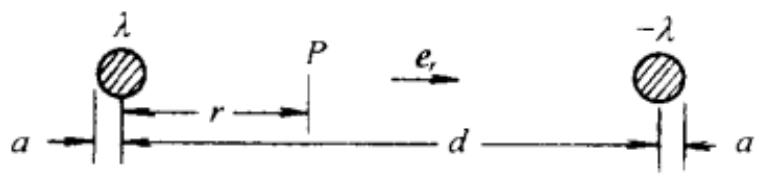
\includegraphics[width=0.5\linewidth]{figures/fig_2_3_35.jpg}
\end{center}

\vfill

\textbf{2.3.36.} 某仪器中有两条长都是 $10\mathrm{cm}$ 的平行直导线，半径都是 $0.1\mathrm{mm}$ ，中心相距为 $1.0\mathrm{mm}$ ，试估算它们之间的电容。

\vfill

\newpage

\textbf{2.3.37.} 四个电容器的电容分别为 $C_1, C_2, C_3$ 和 $C_4$ , 联接如图 2.3.37 所示. 试求: (1) $A, B$ 间的电容 $C_{AB}$ ; (2) $D, E$ 间的电容 $C_{DE}$ ; (3) $A, E$ 间的电容 $C_{AE}$ .

\vfill

\textbf{2.3.38.} 四个电容器的电容都是 $C$ ，分别联接成图2.3.38的(1)和(2). 试分别求两图中 $A, B$ 间的电容.


图2.3.38
\begin{center}
    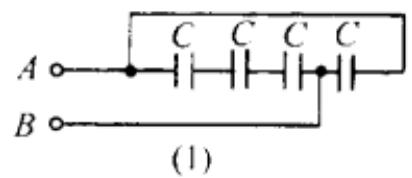
\includegraphics[width=0.5\linewidth]{figures/fig_2_3_38_1.jpg}
\end{center}
\begin{center}
    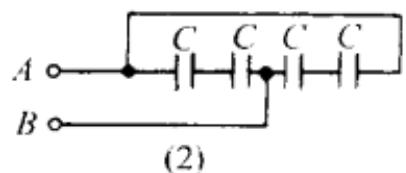
\includegraphics[width=0.5\linewidth]{figures/fig_2_3_38_2.jpg}
\end{center}

\vfill

\newpage

\textbf{2.3.39.} 四个电容 $C_{1}$ 、 $C_{2}$ 、 $C_{3}$ 和 $C_{4}$ 都已知，试分别求图 2.3.39 中两种联法时(1)A、B 间的电容 $C_{AB}$ 和 (2)E、D 间的电容 $C_{ED}$ .

\vfill

\textbf{2.3.40.} 一标准电容箱内有六个标准电容,其联接线路如图 2.3.40 所示. 图中数字是电容的值,单位是微法( $\mu F$ );K $_{1}$ 至 K $_{7}$ 是七个单刀双掷开关,每个都可接

图2.3.40

到上边, 也可以接到下边, 还可以上下都不接. 利用这些开关的不同接法, 就可以在 $A, B$ 间得到各种数值的标准电容. (1) 当 $\mathrm{K}_4$ 和 $\mathrm{K}_6$ 都接到上边, $\mathrm{K}_5$ 和 $\mathrm{K}_7$ 都接到下边, 而其他 $K$ 上下都不接时, $A, B$ 间的电容是多少? (2) $\mathrm{K}_1$ 接到上边, $\mathrm{K}_3$ 接到下边, 其余 $K$ 上下都不接时, $A, B$ 间的电容是多少? (3) 要得 $0.4\mu F$ 的电容, 各 $K$ 如何接? (4) 能得到的最大电容是多少? 如何接? (5) 能得到的最小电容是多少? 如何接?
\begin{center}
    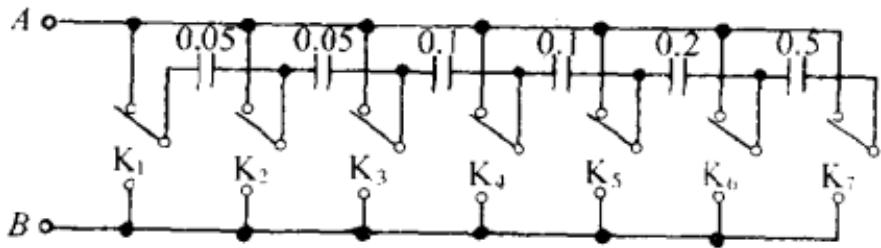
\includegraphics[width=0.5\linewidth]{figures/fig_2_3_40.jpg}
\end{center}

\vfill

\newpage

\textbf{2.3.41.} 五个电容联接如图 2.3.41(1)，已知 $C_{1}=C_{3}=C_{4}=C_{5}=4.0\mu F, C_{2}=1.0\mu F$ ，试求 A、B 间的电容.

\vfill

\textbf{2.3.42.} 五个电容联接如图 2.3.42, 它们的电容 $C_{1}$ 、 $C_{2}$ 、 $C_{3}$ 、 $C_{4}$ 和 $C_{5}$ 都已知, 试求 a、b 间的电容 $C_{ab}$ .

\vfill

\newpage

\textbf{2.3.43.} 三个电容联接如图 2.3.43(1)，已知 $C_{1}=0.25\mu F, C_{2}=0.15\mu F, C_{3}=0.20\mu F, C_{1}$ 上的电压为 50 伏，试求 A、B 间的电压 $U_{AB}$ .

图2.3.43(1)

图2.3.43(2)
\begin{center}
    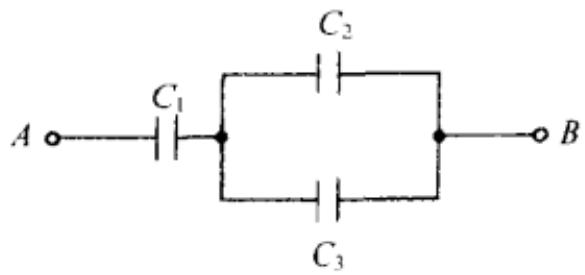
\includegraphics[width=0.5\linewidth]{figures/fig_2_3_43_1.jpg}
\end{center}
\begin{center}
    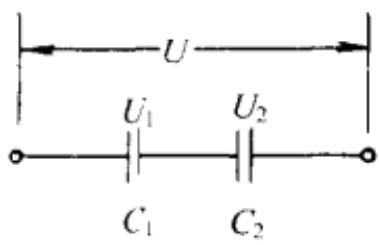
\includegraphics[width=0.5\linewidth]{figures/fig_2_3_43_2.jpg}
\end{center}

\vfill

\textbf{2.3.44.} $C_{1}=0.50\mu F$ 和 $C_{2}=0.20\mu F$ 的两电容串联后，加上220伏的电压，试求每个电容上的电荷量和电压.

\vfill

\newpage

\textbf{2.3.45.} 两个电容器, $C_1 = 1.0\mu \mathrm{F}, C_2 = 10\mu \mathrm{F}$ , 原来都不带电, 串联后接到电池上, 电池的两极对于地的电势分别为 $-100\mathrm{V}$ 和 $+100\mathrm{V}$ , 如图2.3.45所示. 现在接通电键K, 使联接 $C_1$ 和 $C_2$ 的导线接地, 试求通过K的电荷量.

图2.3.45

\vfill

\textbf{2.3.46.} 三个已知的电容 $C_1, C_2$ 和 $C_3$ 都不带电，联接如图2.3.46所示。先将K接到 $a$ ，使 $C_1$ 充电到电压为 $U$ ；然后将K拨到 $b$ ，试求最后各电容器上的电荷量。
\begin{center}
    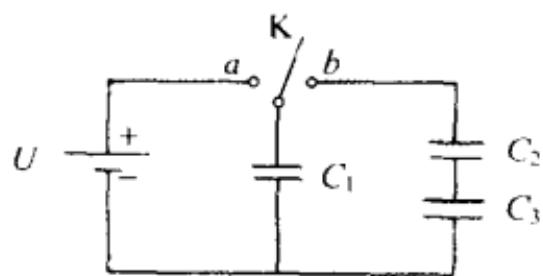
\includegraphics[width=0.5\linewidth]{figures/fig_2_3_46.jpg}
\end{center}

\vfill

\newpage

\textbf{2.3.47.} 四个电容器, $C_{1}=C_{4}=0.20\mu F$ , $C_{2}=C_{3}=0.60\mu F$ ,联接如图2.3.47所示.(1)试分别求K断开和接通时的 $C_{ab}$ ;(2)当 $U_{ab}=100V$ 时,试分别求K断开和接通时各电容上的电压.

\vfill

\textbf{2.3.48.} 如图 2.3.48, $C_{1}=20\mu F$ , $C_{2}=5\mu F$ , 先用 U=1000V 使 $C_{1}$ 充电, 然后将 K 拨到另一侧使 $C_{1}$ 与 $C_{2}$ 联接. 试求: (1) $C_{1}$ 和 $C_{2}$ 各带的电荷量 $Q_{1}$ 和 $Q_{2}$ ; (2) $C_{1}$ 和 $C_{2}$ 各自的电压 $U_{1}$ 和 $U_{2}$ .

\vfill

\newpage

\textbf{2.3.49.} 如图 2.3.49, $C_{1}=3.0\mu F$ , $C_{2}=4.0\mu F$ , $C_{3}=2.0\mu F$ , $U_{a}=120V$ , c 点接地(电势为零). 试求各电容上的电荷量和 b 点的电势 $U_{b}$ .

\vfill

\textbf{2.3.50.} 图 2.3.50 中 $C_{1}=C_{2}=C_{3}=C_{4}$ ，电源的电动势为 9.0V。试求下列两种情况下各电容器上的电压：(1) $K_{2}$ 先是断开的，接通 $K_{1}$ ，使电容器充完电，然后断开 $K_{1}$ ，再接通 $K_{2}$ ；(2) 先接通 $K_{1}$ ，再接通 $K_{2}$ ，使电容器都充完电，然后断开 $K_{1}$ 。

\vfill

\newpage

\textbf{2.3.51.} 两个电容器分别充电到不同的电压, 已知 $C_{1} = 2.0 \mu \mathrm{F}, U_{1} = 400 \mathrm{~V}$ ; $C_{2} = 1.0 \mu \mathrm{F}, U_{2} = 500 \mathrm{~V}$ . 断开电源后, 将 $C_{1}$ 的正极板与 $C_{2}$ 的负极板联接, $C_{1}$ 的负极板与 $C_{2}$ 的正极板联接. 试求: (1) $C_{1}$ 和 $C_{2}$ 上的电荷量; (2) $C_{1}$ 和 $C_{2}$ 上的电压.

\vfill

\textbf{2.3.52.} 图 2.3.52 中的电容 $C_{1}$ 、 $C_{2}$ 、 $C_{3}$ 都是已知，电容 $C_{4}$ 的值是可以调节的。问当 $C_{4}$ 调节到 A、B 两点的电势相等时， $C_{4}$ 的值是多少？

\vfill

\newpage

\textbf{2.3.53.} 两个相同的空气电容器并联后,加上电压 $U_{ab}=U$ . 断开电源后,在其中一个电容器的两极板间充满电容率为 $\varepsilon$ 的均匀介质,如图2.3.53所示.试求这时的 $U_{ab}$ .

\vfill

\textbf{2.3.54.} 两个相同的空气电容器,串联后接到电压为 U 的电源上,再将其中一个电容器两极板间充满电容率为 $\varepsilon$ 的均匀介质,如图 2.3.54 所示,电源的负极接地(电势为零).试求放入介质前后两电容器间联线 a 的电势变化.

图2.3.54
\begin{center}
    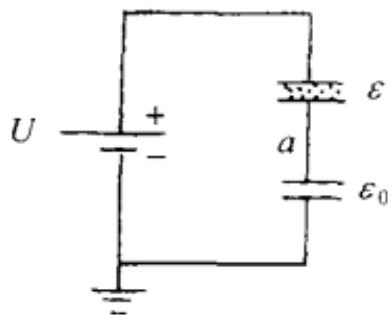
\includegraphics[width=0.5\linewidth]{figures/fig_2_3_54.jpg}
\end{center}

\vfill

\newpage

\textbf{2.3.55.} 将 $C_1 = 1.0\mu \mathrm{F}$ 和 $C_2 = 2.0\mu \mathrm{F}$ 的两个电容器并联后接到 $900\mathrm{V}$ 的直流电源上. (1)试求每个电容器上的电压和电荷量; (2)断开电源, 并将 $C_1$ 和 $C_2$ 彼此断开, 然后再将它们带异号电荷的极板分别接在一起, 试求每个电容器上的电压和电荷量.

\vfill

\textbf{2.3.56.} 将 $C_1 = 2.0\mu \mathrm{F}$ 和 $C_2 = 8.0\mu \mathrm{F}$ 的两个电容器串联后，在两端加上300伏的直流电压。（1）试求每个电容器上的电荷量和电压；(2)断开电源，并将 $C_1$ 和 $C_2$ 彼此断开，然后再将它们带正电荷的两极板接在一起，带负电荷的两极板也接在一起，试求每个电容器上的电荷量和电压；(3)如果断开电源并彼此断开后，再将它们带异号电荷的极板分别接在一起,试求每个电容器上的电荷量和电压.

\vfill

\newpage

\textbf{2.3.57.} $C_1 = 100\mathrm{pF}$ 的电容器充电到 $50\mathrm{V}$ 后断开电源，再将它的两极板分别接到另一电容器 $C_2$ 的两极板上， $C_2$ 原来不带电。接好测得 $C_1$ 上的电压降低为 $35\mathrm{V}$ 。试求 $C_2$ 的值。

\vfill

\textbf{2.3.58.} 有一些相同的电容器, 每个的电容都是 $2.0 \mu \mathrm{F}$ , 耐压都是 $200 \mathrm{~V}$ . 现在要用它们联接成能耐压 $1000 \mathrm{~V}$ 的 (1) $C = 0.40 \mu \mathrm{F}$ 和 (2) $C' = 1.2 \mu \mathrm{F}$ 的电容器, 问各需这种电容器多少个? 怎样联法?

【解答】（1）五个串联，可耐压 $5 \times 200 = 1000\mathrm{V}$ ；电容为 $C = \frac{2.0}{5} = 0.40\mu \mathrm{F}$ ，符合要求。

(2)要耐压 1000V, 必须五个串联; 同时要求 $C' = 1.2\mu F$ , 故须将三个串联再并联起来, 才能达到 $1.2\mu F$ . 因此, 用 15 个这种电容器, 每五个串联后, 三个串联再并联, 便符合要求.

图2.3.59
\begin{center}
    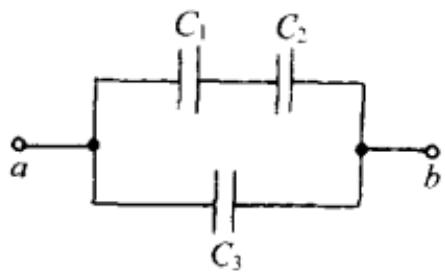
\includegraphics[width=0.5\linewidth]{figures/fig_2_3_58.jpg}
\end{center}

\vfill

\newpage

\textbf{2.3.59.} 三个电容器联接如图 2.3.59, 已知 $C_{1}=100\mu F, C_{2}=25\mu F, C_{3}=30\mu F, U_{ab}=100V$ . 试求每个电容器上的电压和电荷量.

\vfill

\textbf{2.3.60.} 一空气平行板电容器两极板的面积都是 S，相距为 d，电容便为 C=$\frac{\varepsilon_0S}{d}$ 当在两极板加上电压 $U$ 时，略去边缘效应，两极板间电场强度 $\pmb{E}$ 的大小便为 $E = U / d$ 其中一板上的电荷量为 $Q = CU$ ，故它所受的力的大小为

$$
F = Q E = C U \left(\frac {U}{d}\right) = \frac {C U ^ {2}}{d}
$$

你认为这个结果对不对？为什么？

【解答】不对. 因为 $E = U / d$ 是两极板间的电场强度, 而不是面电荷 $Q$ 所在处的电场强度. $Q$ 所在处的电场强度的大小为

$$
E _ {Q} = \frac {1}{2} E = \frac {U}{2 d}
$$

故正确的结果应为

$$
F = Q E _ {Q} = \frac {Q U}{2 d} = \frac {C U ^ {2}}{2 d}
$$

\vfill

\newpage

\textbf{2.3.61.} 一平行板电容器两极板的面积都是 S，相距为 d，两板间是空气。略去边缘效应。(1) 当两极板的电压为 U 时，试求它们之间相互作用的静电力 F 的大小 F；(2) 当 $S = 100 ~mm^{2}$ ，d = 1.0 mm，U = 2000 V 时，计算 F 的值。

\vfill

\textbf{2.3.62.} 一平行板电容器两极板间充满均匀介质，其介电常数为 $\varepsilon_{\mathrm{r}} = 2.0$ ，电介质强度为 $E_{m} = 1.0\times 10^{9}\mathrm{V / m}$ 略去边缘效应．试求介质在将要击穿时所受的静电压强(静电力所产生的压强).

\vfill

\newpage

\textbf{2.3.63.} 静电天平的原理如图 2.3.63 所示,一空气平行板电容器两极板的面

图2.3.63

积都是 S，相距为 x，下板固定，上板接到天平的一端。当电容器不带电时，天平正好平衡。然后在电容器的两极板上加电压 U，则天平的另一端必须加上质量为 m 的砝码，才能达到平衡。略去边缘效应。试求所加的电压 U。
\begin{center}
    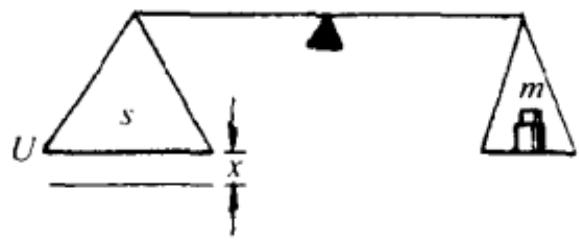
\includegraphics[width=0.5\linewidth]{figures/fig_2_3_63.jpg}
\end{center}

\vfill

\textbf{2.3.64.} 空气能承受的电场强度的最大值(称为电介质强度)为 $E_{m}=30kV/cm$ ，超过这个数值，空气就要被击穿，发生火花放电。今有一平行板电容器，两极板相距为 0.50cm，极板间是空气。略去边缘效应。试问它能耐多高的电压？

\vfill

\newpage

\textbf{2.3.65.} 空气的电介质强度为 $E_{m}=3000kV/m$ ，当空气平行板电容器两极板

的电势差为 50kV 时, 略去边缘效应, 试问单位面积上的电容最大是多少?

\vfill

\textbf{2.3.66.} 两个电容器上分别标明: $C_1:200\mathrm{pF}500\mathrm{V}; C_2:300\mathrm{pF}900\mathrm{V}$ . 将它们串联后, 加上 $1000\mathrm{V}$ 电压, 是否会被击穿?

\vfill

\newpage

\textbf{2.3.67.} 两个电容器上分别标明: $C_1$ 耐压 $V_1, C_2$ 耐压 $V_2$ . 现将它们串联后, 加上电压 $U$ , 如图 2.3.67 所示. 使 $U$ 逐渐升高, 问哪个电容先被击穿? 为什么?
\begin{center}
    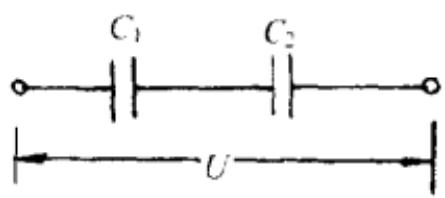
\includegraphics[width=0.5\linewidth]{figures/fig_2_3_67.jpg}
\end{center}

\vfill

\textbf{2.3.68.} 三个电容器联接如图2.3.68所示，它们的电容值已在图中标出。（1）试求 $A, B$ 间的电容 $C_{AB}$ ；（2）在 $A, B$ 间加上100伏的电压，试求 $C_1$ 上的电荷量 $Q_1$ 和电压 $U_1$ ；（3）如果这时 $C$ 被击穿（即变成通路），问 $C_1$ 上的电荷量和电压各是多少？

图2.3.68

$$
\begin{array}{r l} & {\text {【解】}} \\ & {(1) C _ {A B} = \frac {C (C _ {1} + C _ {2})}{C + C _ {1} + C _ {2}} = \frac {4 \times (1 0 + 5)}{4 + 1 0 + 5} = 3. 2 (\mu \mathrm{F})} \\ & {(2) U _ {1} = \frac {C}{C _ {1} + C _ {2} + C} U = \frac {4}{1 0 + 5 + 4} \times 1 0 0 = 2 1 (\mathrm{V})} \\ & {\qquad Q _ {1} = C _ {1} U _ {1} = 1 0 \times 1 0 ^ {- 6} \times 2 1 = 2. 1 \times 1 0 ^ {- 4} (\mathrm{C})} \end{array}
$$

(3) $C$ 被击穿, 即变成通路, 这时 $100\mathrm{V}$ 的电压便都加 $C_1$ 和 $C_2$ 的并联上, 故 $C_1$ 上的电压和电荷量分别为

$$
\begin{array}{r l} & U _ {1} ^ {\prime} = U = 1 0 0 \mathrm{V} \\ & Q _ {1} ^ {\prime} = C _ {1} U _ {1} ^ {\prime} = 1 0 \times 1 0 ^ {- 6} \times 1 0 0 = 1. 0 \times 1 0 ^ {- 3} (\mathrm{C}) \end{array}
$$

\vfill

\newpage

\textbf{2.3.69.} 一圆柱电容器由直径为 $5.0\mathrm{mm}$ 的直导线和与它共轴的直圆筒构成，圆筒的内直径为 $5.0\mathrm{cm}$ ，导线与圆筒间是空气。已知空气的电介质强度为 $30\mathrm{kV/cm}$ ，试问这电容器能耐多高的电压？

\vfill

\textbf{2.3.70.} 共轴的两导体圆筒, 内筒的外半径为 $R_{1}$ , 外筒的内半径为 $R_{2}(R_{2}<2R_{1})$ , 其间有两层均匀介质, 内层的电容率为 $\varepsilon_{1}$ , 外层的电容率为 $\varepsilon_{2}=\varepsilon_{1}/2$ , 它们的交界面是半径为 $R$ 的圆柱面. 已知这两介质的电介质强度都是 $E_{m}$ . 试证明: 两筒间的最大电势差为 $U_{m}=\frac{1}{2}RE_{m}\ln(R_{2}^{2}/RR_{1})$ .

\vfill

\newpage

\textbf{2.3.71.} 一圆柱电容器内充满两层均匀介质, 内层是 $\varepsilon_{r1} = 4.0$ 的油纸, 其内半径为 $2.0\mathrm{cm}$ , 外半径为 $2.3\mathrm{cm}$ ; 外层是 $\varepsilon_{r2} = 7.0$ 的玻璃, 其外半径为 $2.5\mathrm{cm}$ . 已知油纸的电介质强度为 $120\mathrm{kV/cm}$ , 玻璃的电介质强度为 $100\mathrm{kV/cm}$ , 试问这电容器能耐多高的电压? 当电压逐渐升高时, 哪层介质先被击穿?

\vfill

\textbf{2.3.72.} 一同轴电缆里面导体的半径为 $R_{1}$ , 外面导体的内半径为 $R_{3}$ , 两导体间充满了两层均匀介质, 它们的交界面是 $R_{2}$ , 内外两层介质的电容率分别为 $\varepsilon_{1}$ 和 $\varepsilon_{2}$ , 其横截面如图 2.3.72 所示. 已知两介质的电介质强度分别为 $E_{1}$ 和 $E_{2}$ . 试证明: 当两极 (即内外两导体) 间的电压逐渐升高时, 在 $\varepsilon_{1} R_{1} E_{1} > \varepsilon_{2} R_{2} E_{2}$ 的条件下, 首先被击穿的是外层电介质.

图2.3.72

高斯定理得,两介质内电场强度的表达式分别为

$$
\boldsymbol {E} _ {1} = \frac {\lambda}{2 \pi \epsilon_ {1} r} \boldsymbol {e} _ {r}, \quad \boldsymbol {E} _ {2} = \frac {\lambda}{2 \pi \epsilon_ {2} r} \boldsymbol {e} _ {r}\tag{1}
$$

式中 $e_r = \frac{r}{r}, r$ 是从轴线到场点的位矢。由式(1)得每个介质能承受的 $\lambda_{\max}$ 分别为

$$
\lambda_ {1 \max} = 2 \pi \varepsilon_ {1} R _ {1} E _ {1 \max} = 2 \pi \varepsilon_ {1} R _ {1} E _ {1}\tag{2}
$$

$$
\lambda_ {2 \max} = 2 \pi \varepsilon_ {2} R _ {2} E _ {2 \max} = 2 \pi \varepsilon_ {2} R _ {2} E _ {2}\tag{3}
$$

若

$$
\lambda_ {2 \max} <   \lambda_ {1 \max}\tag{4}
$$

则 $\varepsilon_{2}$ (外层介质) 首先被击穿, 将式(2)、(3)代入式(4)即得

$$
\varepsilon_ {1} R _ {1} E _ {1} > \varepsilon_ {2} R _ {2} E _ {2}\tag{5}
$$

\vfill

\newpage
